% Презентація: етап «Вибір теми командного проєкту»
% Збирання: make pdf (слайди) | make notes (слайди з нотатками) | make clean
\documentclass[aspectratio=169,xcolor=table]{beamer}

% Нотатки доповідача: main-notes.tex визначає \shownotes перед % Презентація: етап «Вибір теми командного проєкту»
% Збирання: make pdf (слайди) | make notes (слайди з нотатками) | make clean
\documentclass[aspectratio=169,xcolor=table]{beamer}

% Нотатки доповідача: main-notes.tex визначає \shownotes перед % Презентація: етап «Вибір теми командного проєкту»
% Збирання: make pdf (слайди) | make notes (слайди з нотатками) | make clean
\documentclass[aspectratio=169,xcolor=table]{beamer}

% Нотатки доповідача: main-notes.tex визначає \shownotes перед % Презентація: етап «Вибір теми командного проєкту»
% Збирання: make pdf (слайди) | make notes (слайди з нотатками) | make clean
\documentclass[aspectratio=169,xcolor=table]{beamer}

% Нотатки доповідача: main-notes.tex визначає \shownotes перед \input{main}
\ifdefined\shownotes
  \usepackage{pgfpages}
  \setbeameroption{show notes on second screen=right}
  % XeLaTeX + pgfpages: після кольорового тексту колір не відновлюється
  % (основний текст стає білим). Переводимо кольори на pdfcolorstack,
  % який після кожного pop явно повертає поточний колір.
  \makeatletter
  \def\nt@conv#1 #2\@nil{\csname nt@conv@#1\endcsname#2\@nil}
  \def\nt@conv@rgb#1 #2 #3\@nil{#1 #2 #3 rg #1 #2 #3 RG}
  \def\nt@conv@gray#1\@nil{#1 g #1 G}
  \def\nt@conv@cmyk#1 #2 #3 #4\@nil{#1 #2 #3 #4 k #1 #2 #3 #4 K}
  \AtBeginDocument{%
    \special{pdfcolorstackinit 1 page direct (0 g 0 G)}%
    \def\beamerorig@set@color{%
      \edef\nt@tmp{\current@color\space}%
      \special{pdfcolorstack 1 push (\expandafter\nt@conv\nt@tmp\@nil)}%
      \aftergroup\reset@color}%
    \def\beamerorig@reset@color{%
      \special{pdfcolorstack 1 pop}\special{pdfcolorstack 1 current}}%
  }
  \makeatother
\fi

% ---------- Тема ----------
\usetheme[progressbar=frametitle,numbering=counter]{metropolis}
\setbeamertemplate{navigation symbols}{}

% ---------- Кольори (усе в одному місці) ----------
\definecolor{accent}{HTML}{C8461B}   % акцент
\definecolor{ink}{HTML}{23272B}      % темний нейтральний
\colorlet{swotS}{accent}
\colorlet{swotO}{accent!70!black}
\colorlet{swotW}{ink}
\colorlet{swotT}{ink!60}
\colorlet{highlight}{accent!15}

\setbeamercolor{frametitle}{bg=ink,fg=white}
\setbeamercolor{progress bar}{fg=accent,bg=accent!20}
\setbeamercolor{title separator}{fg=accent}
\setbeamercolor{alerted text}{fg=accent}
\setbeamercolor{background canvas}{bg=white}
\setbeamercolor{normal text}{fg=ink}
\setbeamercolor{standout}{bg=ink,fg=white}
\setbeamercolor{itemize item}{fg=accent}
\setbeamercolor{enumerate item}{fg=accent}

% ---------- Мова і шрифти ----------
\usepackage{fontspec}
\usepackage{polyglossia}
\setdefaultlanguage{ukrainian}
\setotherlanguage{english}
% PT Sans з TeX Live (пакет paratype), підключений за іменами файлів
\defaultfontfeatures{Ligatures=TeX}
\setmainfont{PTS55F.ttf}[BoldFont=PTS75F.ttf,ItalicFont=PTS56F.ttf,BoldItalicFont=PTS76F.ttf]
\setsansfont{PTS55F.ttf}[BoldFont=PTS75F.ttf,ItalicFont=PTS56F.ttf,BoldItalicFont=PTS76F.ttf]
\newfontfamily\cyrillicfont{PTS55F.ttf}[BoldFont=PTS75F.ttf,ItalicFont=PTS56F.ttf,BoldItalicFont=PTS76F.ttf]
\newfontfamily\cyrillicfontsf{PTS55F.ttf}[BoldFont=PTS75F.ttf,ItalicFont=PTS56F.ttf,BoldItalicFont=PTS76F.ttf]
\setmonofont{PTM55F.ttf}[Scale=MatchLowercase]
\setbeamerfont{frametitle}{series=\bfseries}
\setbeamerfont{title}{series=\bfseries}

% ---------- Пакети ----------
\usepackage{booktabs}
\usepackage{array}
\usepackage{tabularx}
\usepackage{graphicx}
\usepackage{tikz}
\usetikzlibrary{positioning,arrows.meta}
\usepackage[most]{tcolorbox}

\renewcommand{\arraystretch}{1.25}

% SWOT-квадрант: #1 колір, #2 літера, #3 підпис, #4 пункти, #5 група рівної висоти
\newcommand{\swotbox}[5]{%
  \begin{tcolorbox}[enhanced,colframe=#1,colback=#1!7,boxrule=0.6pt,arc=2pt,
    equal height group=#5,left=4pt,right=4pt,top=2pt,bottom=2pt,
    fonttitle=\bfseries\small,coltitle=white,colbacktitle=#1,
    toptitle=1pt,bottomtitle=1pt,
    title={\large #2\enspace\normalsize\mdseries #3}]
    \small\setlength{\leftmargini}{1.1em}
    \begin{itemize}\setlength{\itemsep}{1pt}
      #4
    \end{itemize}
  \end{tcolorbox}}

\newcommand{\swotgrid}[4]{%
  \begin{columns}[T,onlytextwidth]
    \begin{column}{0.49\textwidth}
      \swotbox{swotS}{S}{Сильні сторони}{#1}{swottop}\vspace{-4pt}
      \swotbox{swotO}{O}{Можливості}{#3}{swotbottom}
    \end{column}
    \begin{column}{0.49\textwidth}
      \swotbox{swotW}{W}{Слабкі сторони}{#2}{swottop}\vspace{-4pt}
      \swotbox{swotT}{T}{Загрози}{#4}{swotbottom}
    \end{column}
  \end{columns}}

% ---------- Титульні дані ----------
\title{Вибір теми командного проєкту}
\subtitle{Обрана тема: «Цифровий тренер для автоспорту»}
\date{}

\begin{document}

\input{slides/intro}
\input{slides/topics}
\input{slides/swot}
\input{slides/comparison}
\input{slides/decision}
\input{slides/next-steps}

\end{document}

\ifdefined\shownotes
  \usepackage{pgfpages}
  \setbeameroption{show notes on second screen=right}
  % XeLaTeX + pgfpages: після кольорового тексту колір не відновлюється
  % (основний текст стає білим). Переводимо кольори на pdfcolorstack,
  % який після кожного pop явно повертає поточний колір.
  \makeatletter
  \def\nt@conv#1 #2\@nil{\csname nt@conv@#1\endcsname#2\@nil}
  \def\nt@conv@rgb#1 #2 #3\@nil{#1 #2 #3 rg #1 #2 #3 RG}
  \def\nt@conv@gray#1\@nil{#1 g #1 G}
  \def\nt@conv@cmyk#1 #2 #3 #4\@nil{#1 #2 #3 #4 k #1 #2 #3 #4 K}
  \AtBeginDocument{%
    \special{pdfcolorstackinit 1 page direct (0 g 0 G)}%
    \def\beamerorig@set@color{%
      \edef\nt@tmp{\current@color\space}%
      \special{pdfcolorstack 1 push (\expandafter\nt@conv\nt@tmp\@nil)}%
      \aftergroup\reset@color}%
    \def\beamerorig@reset@color{%
      \special{pdfcolorstack 1 pop}\special{pdfcolorstack 1 current}}%
  }
  \makeatother
\fi

% ---------- Тема ----------
\usetheme[progressbar=frametitle,numbering=counter]{metropolis}
\setbeamertemplate{navigation symbols}{}

% ---------- Кольори (усе в одному місці) ----------
\definecolor{accent}{HTML}{C8461B}   % акцент
\definecolor{ink}{HTML}{23272B}      % темний нейтральний
\colorlet{swotS}{accent}
\colorlet{swotO}{accent!70!black}
\colorlet{swotW}{ink}
\colorlet{swotT}{ink!60}
\colorlet{highlight}{accent!15}

\setbeamercolor{frametitle}{bg=ink,fg=white}
\setbeamercolor{progress bar}{fg=accent,bg=accent!20}
\setbeamercolor{title separator}{fg=accent}
\setbeamercolor{alerted text}{fg=accent}
\setbeamercolor{background canvas}{bg=white}
\setbeamercolor{normal text}{fg=ink}
\setbeamercolor{standout}{bg=ink,fg=white}
\setbeamercolor{itemize item}{fg=accent}
\setbeamercolor{enumerate item}{fg=accent}

% ---------- Мова і шрифти ----------
\usepackage{fontspec}
\usepackage{polyglossia}
\setdefaultlanguage{ukrainian}
\setotherlanguage{english}
% PT Sans з TeX Live (пакет paratype), підключений за іменами файлів
\defaultfontfeatures{Ligatures=TeX}
\setmainfont{PTS55F.ttf}[BoldFont=PTS75F.ttf,ItalicFont=PTS56F.ttf,BoldItalicFont=PTS76F.ttf]
\setsansfont{PTS55F.ttf}[BoldFont=PTS75F.ttf,ItalicFont=PTS56F.ttf,BoldItalicFont=PTS76F.ttf]
\newfontfamily\cyrillicfont{PTS55F.ttf}[BoldFont=PTS75F.ttf,ItalicFont=PTS56F.ttf,BoldItalicFont=PTS76F.ttf]
\newfontfamily\cyrillicfontsf{PTS55F.ttf}[BoldFont=PTS75F.ttf,ItalicFont=PTS56F.ttf,BoldItalicFont=PTS76F.ttf]
\setmonofont{PTM55F.ttf}[Scale=MatchLowercase]
\setbeamerfont{frametitle}{series=\bfseries}
\setbeamerfont{title}{series=\bfseries}

% ---------- Пакети ----------
\usepackage{booktabs}
\usepackage{array}
\usepackage{tabularx}
\usepackage{graphicx}
\usepackage{tikz}
\usetikzlibrary{positioning,arrows.meta}
\usepackage[most]{tcolorbox}

\renewcommand{\arraystretch}{1.25}

% SWOT-квадрант: #1 колір, #2 літера, #3 підпис, #4 пункти, #5 група рівної висоти
\newcommand{\swotbox}[5]{%
  \begin{tcolorbox}[enhanced,colframe=#1,colback=#1!7,boxrule=0.6pt,arc=2pt,
    equal height group=#5,left=4pt,right=4pt,top=2pt,bottom=2pt,
    fonttitle=\bfseries\small,coltitle=white,colbacktitle=#1,
    toptitle=1pt,bottomtitle=1pt,
    title={\large #2\enspace\normalsize\mdseries #3}]
    \small\setlength{\leftmargini}{1.1em}
    \begin{itemize}\setlength{\itemsep}{1pt}
      #4
    \end{itemize}
  \end{tcolorbox}}

\newcommand{\swotgrid}[4]{%
  \begin{columns}[T,onlytextwidth]
    \begin{column}{0.49\textwidth}
      \swotbox{swotS}{S}{Сильні сторони}{#1}{swottop}\vspace{-4pt}
      \swotbox{swotO}{O}{Можливості}{#3}{swotbottom}
    \end{column}
    \begin{column}{0.49\textwidth}
      \swotbox{swotW}{W}{Слабкі сторони}{#2}{swottop}\vspace{-4pt}
      \swotbox{swotT}{T}{Загрози}{#4}{swotbottom}
    \end{column}
  \end{columns}}

% ---------- Титульні дані ----------
\title{Вибір теми командного проєкту}
\subtitle{Обрана тема: «Цифровий тренер для автоспорту»}
\date{}

\begin{document}

% ===== 1. Титульний =====
\begin{frame}[plain]
  \vspace*{-0.6cm}\titlepage
  \note{[Доповідач 1] Добрий день! Ми сьогодні захищаємо перший етап командного проєкту — вибір теми. Одразу скажемо результат: ми обрали тему «Цифровий тренер для автоспорту». Це вебзастосунок, який перетворює GPS-запис з екшн-камери чи телефона на розбір заїзду з порадами. Але до цього рішення ми дійшли не одразу. Ми розглянули дві ідеї, для кожної написали опис і зробили SWOT-аналіз, а потім порівняли їх за однаковими критеріями. Далі покажемо весь цей шлях по кроках. Говоритимемо по черзі, кожен про свою частину.}
\end{frame}

% ===== 2. Мета і процес =====
\begin{frame}{Мета етапу і як ми обирали тему}
  \textbf{Мета:} обрати тему командного проєкту й обґрунтувати вибір.

  \vspace{1.2em}
  \centering
  \begin{tikzpicture}[
      stp/.style={draw=accent,fill=accent!8,rounded corners=3pt,line width=0.8pt,
        minimum width=2.15cm,minimum height=1.1cm,align=center,font=\small\bfseries},
      final/.style={stp,fill=accent,text=white},
      desc/.style={font=\small,text width=2.3cm,align=center,text=ink!80},
      arr/.style={-{Stealth[length=2.2mm]},line width=0.9pt,draw=ink!60},
      node distance=0.5cm]
    \node[stp] (s1) {Ідеї};
    \node[stp,right=of s1] (s2) {Опис};
    \node[stp,right=of s2] (s3) {SWOT};
    \node[stp,right=of s3] (s4) {Порівняння\\за критеріями};
    \node[final,right=of s4] (s5) {Рішення};
    \foreach \a/\b in {s1/s2,s2/s3,s3/s4,s4/s5} \draw[arr] (\a) -- (\b);
    \node[desc,below=0.3cm of s1] {дві теми};
    \node[desc,below=0.3cm of s2] {що, для кого, яка проблема};
    \node[desc,below=0.3cm of s3] {сильні й слабкі сторони, можливості, загрози};
    \node[desc,below=0.3cm of s4] {5 критеріїв з вагами, оцінки 1–5};
    \node[desc,below=0.3cm of s5] {цифровий тренер для автоспорту};
  \end{tikzpicture}

  \note{[Доповідач 1] Мета етапу — не просто назвати тему, а обґрунтувати, чому саме її. Тому ми йшли за простою схемою з п'яти кроків. Спочатку зібрали ідеї: у підсумку їх дві — цифровий тренер для автоспорту і розумний кошик для товарів. Для кожної написали опис: що це, для кого і яку проблему вирішує. Потім зробили SWOT-аналіз із джерелами. Далі домовилися про п'ять критеріїв з вагами і поставили кожній темі оцінки від одного до п'яти. І лише після цього ухвалили рішення. Так обидві теми ми порівнювали за однаковими правилами, а не за враженням.}
\end{frame}

% ===== 3. Тема 1 =====
\begin{frame}{Тема 1. Цифровий тренер для автоспорту}
  \begin{columns}[T,onlytextwidth]
    \begin{column}{0.48\textwidth}
      \textbf{\color{accent}Призначення}\\
      Вебзастосунок: GPS-запис з камери чи телефона $\to$ розбір заїзду

      \medskip
      \textbf{\color{accent}Для кого}\\
      Новачки й аматори без тренера: прокатний картинг, трек-дні

      \medskip
      \textbf{\color{accent}Проблема}\\
      Немає об'єктивного зворотного зв'язку, тренер і телеметрія дорогі
    \end{column}
    \begin{column}{0.48\textwidth}
      \textbf{\color{accent}Основні можливості}
      \begin{itemize}
        \item Автоматичний поділ заїзду на кола
        \item Траєкторія на карті траси з межами
        \item Повороти, де втрачається найбільше часу
        \item 2–3 поради простою мовою з відео
      \end{itemize}
    \end{column}
  \end{columns}

  \note{[Доповідач 1] Перша тема — цифровий тренер для автоспорту. Уявіть новачка, який регулярно їздить на прокатний картинг. Він відчуває, що десь втрачає час, але не знає, де саме і що змінити. Живий тренер дорогий, а професійна телеметрія розрахована на досвідчених пілотів. Наш застосунок бере запис з екшн-камери GoPro чи трек із телефона, сам ділить заїзд на кола, накладає траєкторію на реальні межі траси і знаходить повороти, де пілот втрачає найбільше часу. На виході — не графіки, а дві-три поради простою мовою з цифрами і фрагментом відео, плюс план на наступний заїзд.}
\end{frame}

% ===== 4. Тема 2 =====
\begin{frame}{Тема 2. Розумний кошик для товарів}
  \begin{columns}[T,onlytextwidth]
    \begin{column}{0.48\textwidth}
      \textbf{\color{accent}Призначення}\\
      Окремий застосунок сам складає кошик у Сільпо через MCP

      \medskip
      \textbf{\color{accent}Для кого}\\
      Зайняті люди 22–40 років у великих містах, клієнти Сільпо

      \medskip
      \textbf{\color{accent}Проблема}\\
      Планувати їжу й покупки щодня — рутина, продукти викидають
    \end{column}
    \begin{column}{0.48\textwidth}
      \textbf{\color{accent}Основні можливості}
      \begin{itemize}
        \item Оцінка того, що є вдома, за історією покупок
        \item План харчування на 2–3 дні
        \item Автоматичний кошик із поясненнями
        \item Підтвердження, доставка чи самовивіз
      \end{itemize}
    \end{column}
  \end{columns}

  \note{[Доповідач 2] Друга тема — розумний кошик для товарів. Ідея така: застосунок сам складає замовлення в Сільпо на найближчі дні. Він знає, що людина зазвичай купує, за історією покупок оцінює, що вже закінчилося вдома, і пропонує простий план харчування на два-три дні. Увечері людина отримує готовий кошик, де біля кожного товару написана причина. Їй лишається переглянути його і обрати доставку чи самовивіз. Працює це через офіційний MCP-сервер, який Сільпо відкрило в серпні 2026 року. Аудиторія — зайняті люди 22–40 років у великих містах, які вже купують у Сільпо.}
\end{frame}

% ===== 5. SWOT: цифровий тренер =====
\begin{frame}{SWOT: цифровий тренер для автоспорту}
  \swotgrid
    {\item Не потрібне нове обладнання
     \item Відкритий формат GPMF і бібліотеки
     \item Демо: середня похибка кола 0,035 с}
    {\item GPS у телефоні: точність \textasciitilde{}4,9 м
     \item Криті картодроми без GPS
     \item Межі траси з відео поки не будуються}
    {\item Живий тренер — €250–350 на день
     \item Track Titan: 200\,000+ користувачів
     \item Ріст картингу: K1 Speed — 107 локацій}
    {\item Tenth Finder і Kart Track дають поради
     \item Дешевий RaceChrono Pro за \$19.99
     \item Камери без GPS, як HERO12}

  \note{[Доповідач 2] Тепер SWOT цифрового тренера. Головна сила — пілоту не треба купувати нове обладнання, досить камери чи телефона. GoPro зберігає телеметрію у відкритому форматі GPMF, і для нього вже є бібліотеки. А наше демо на реальній сесії показало, що час кола за GPS відрізняється від офіційного хронометражу в середньому на 0,035 секунди. Слабкі місця — точність GPS у телефоні, криті картодроми без сигналу і межі траси, які з відео поки не будуються. Можливості — дорогі живі тренери й інвестиції в Track Titan. Загрози — конкуренти, які вже дають поради, дешевий RaceChrono і те, що Камери без GPS, як HERO12.}
\end{frame}

% ===== 6. SWOT: розумний кошик =====
\begin{frame}{SWOT: розумний кошик для товарів}
  \swotgrid
    {\item Офіційний MCP: 40 інструментів
     \item Історія покупок онлайн і в магазинах
     \item Сам пропонує кошик, не чекає запиту}
    {\item «Що є вдома» — лише здогадка
     \item Кошик помиляється з фасуваннями
     \item Усі дані належать Сільпо}
    {\item 81\% купують продукти в магазинах
     \item Вибір страв: десятки хв на тиждень
     \item Відходи: 79 кг їжі на людину на рік}
    {\item Сільпо може зробити те саме
     \item Залежність від правил одного MCP
     \item Харчові дані можуть бути чутливими}

  \note{[Доповідач 2] SWOT розумного кошика. Сильна сторона — офіційний доступ до Сільпо: сорок інструментів, вхід через OAuth і приклади коду. До того ж видно історію покупок не лише онлайн, а й у магазинах. І продукт сам приходить з кошиком, а не чекає запиту. Але оцінка того, що є вдома, — лише здогадка, а в тестах автоматичний кошик уже помилявся з фасуваннями й наявністю. Власних даних у нас немає. Можливості — 81\% українців досі купують продукти в магазинах, тож онлайну є куди рости, плюс тема харчових відходів. Головні загрози — Сільпо може зробити те саме у своєму застосунку, а ми повністю залежимо від правил одного сервера.}
\end{frame}

% ===== 7. Критерії і ваги =====
\begin{frame}{Критерії і ваги}
  \centering
  \begin{tabular}{@{}l c l@{}}
    \toprule
    \textbf{Критерій} & \textbf{Вага} & \textbf{Що означає} \\
    \midrule
    Актуальність проблеми        & 0,25 & Наскільки проблема важлива для аудиторії \\
    Реалізованість за семестр    & 0,25 & Чи зробимо робочий продукт \\
    Конкурентна перевага         & 0,2  & Чим ми кращі за наявні рішення \\
    Інтерес і досвід команди     & 0,15 & Чи хочемо і чи маємо потрібні знання \\
    Ризики і зовнішні залежності & 0,15 & Менше ризиків — вища оцінка \\
    \midrule
    \textbf{Разом}               & \textbf{1,0} & \\
    \bottomrule
  \end{tabular}

  \note{[Доповідач 3] Щоб порівняти теми чесно, ми домовилися про п'ять критеріїв. Найбільшу вагу, по 0,25, мають актуальність проблеми і реалізованість за семестр. Тобто продукт має бути потрібним, і ми маємо встигнути його зробити. Конкурентна перевага важить 0,2: чим ми кращі за те, що вже є. Інтерес і досвід команди та ризики — по 0,15. Для ризиків шкала обернена: що менше ризиків і зовнішніх залежностей, то вища оцінка. Разом ваги дають одиницю, тож підсумок — це зважена оцінка на тій самій шкалі від одного до п'яти.}
\end{frame}

% ===== 8. Порівняння =====
\begin{frame}{Порівняння тем}
  \centering\renewcommand{\arraystretch}{1.1}
  \begin{tabular}{@{}l c >{\columncolor{highlight}}c c@{}}
    \toprule
    \textbf{Критерій} & \textbf{Вага} & \textbf{\begin{tabular}{@{}c@{}}Цифровий\\тренер\end{tabular}} & \textbf{\begin{tabular}{@{}c@{}}Розумний\\кошик\end{tabular}} \\
    \midrule
    Актуальність проблеми        & 0,25 & 4 & 4 \\
    Реалізованість за семестр    & 0,25 & 4 & 4 \\
    Конкурентна перевага         & 0,2  & 3 & 2 \\
    Інтерес і досвід команди     & 0,15 & ? & ? \\
    Ризики і зовнішні залежності & 0,15 & 3 & 2 \\
    \midrule
    \textbf{Зважена сума без «інтересу»} (макс. 4,25) & 0,85 & \textbf{3,05} & \textbf{2,70} \\
    \bottomrule
  \end{tabular}

  \vspace{0.3em}
  \raggedright\small
  Підсумок = зважена сума + 0,15 × середня оцінка інтересу команди.\\
  Кошик випередить тренера, лише якщо його інтерес вищий хоча б на 3 бали.

  \note{[Доповідач 3] Ось самі оцінки. За актуальністю і реалізованістю теми рівні — обидві по 4. Різниця з'являється в конкурентній перевазі: 3 у тренера проти 2 у кошика. І в ризиках теж 3 проти 2. Оцінки за інтерес команди ми ще не зібрали, тому там знаки питання, і зважену суму рахуємо без цього критерію: максимум тут 4,25. Тренер має 3,05, кошик — 2,70, різниця 0,35 бала. Коли кожен з нас поставить свою оцінку, ми додамо 0,15, помножене на середнє. Кошик виграв би, лише якби ми оцінили його інтерес хоча б на 3 бали вище.}
\end{frame}

% ===== 9. Чому цифровий тренер =====
\newcommand{\argcard}[2]{%
  \begin{tcolorbox}[colframe=accent,colback=accent!6,boxrule=0.6pt,arc=2pt,
    height=2.55cm,valign=top,left=5pt,right=5pt,top=4pt,bottom=4pt]
    \raggedright\textbf{#1}\par\smallskip
    \small #2
  \end{tcolorbox}}

\begin{frame}{Чому цифровий тренер}
  \begin{columns}[T,onlytextwidth]
    \begin{column}{0.49\textwidth}
      \argcard{Працює з тим, що в пілота вже є}
        {Камера чи телефон, а не Garmin Catalyst 2 за \$1,199.99}
      \argcard{Люди готові платити за тренування}
        {Живий тренер — €250–350 на день, Track Titan залучив \$5 млн}
    \end{column}
    \begin{column}{0.49\textwidth}
      \argcard{Дані відкриті й належать пілоту}
        {Формат GPMF у відеофайлі, без API чи дозволу компаній}
      \argcard{Поради, а не графіки}
        {2–3 поради з цифрами й відео для новачка}
    \end{column}
  \end{columns}

  \note{[Доповідач 3] Чому саме цифровий тренер? Перше: він працює з тим, що в пілота вже є, — з камерою чи телефоном, а не з пристроєм на кшталт Garmin Catalyst 2 за \$1,199.99. Друге: дані відкриті. GoPro пише телеметрію у форматі GPMF прямо у відеофайл, і цей файл належить пілоту. Нам не потрібен дозвіл чи API жодної компанії — на відміну від кошика. Третє: люди вже платять за тренування. Живий тренер коштує €250–350 на день, а Track Titan залучив \$5 млн. І четверте: ми закриваємо проміжок між графіками і дорогими пристроями — даємо новачку дві-три поради з цифрами і відео.}
\end{frame}

% ===== 10. Як виглядатиме продукт =====
\begin{frame}{Як виглядатиме продукт}
  \begin{columns}[c,onlytextwidth]
    \begin{column}{0.62\textwidth}
      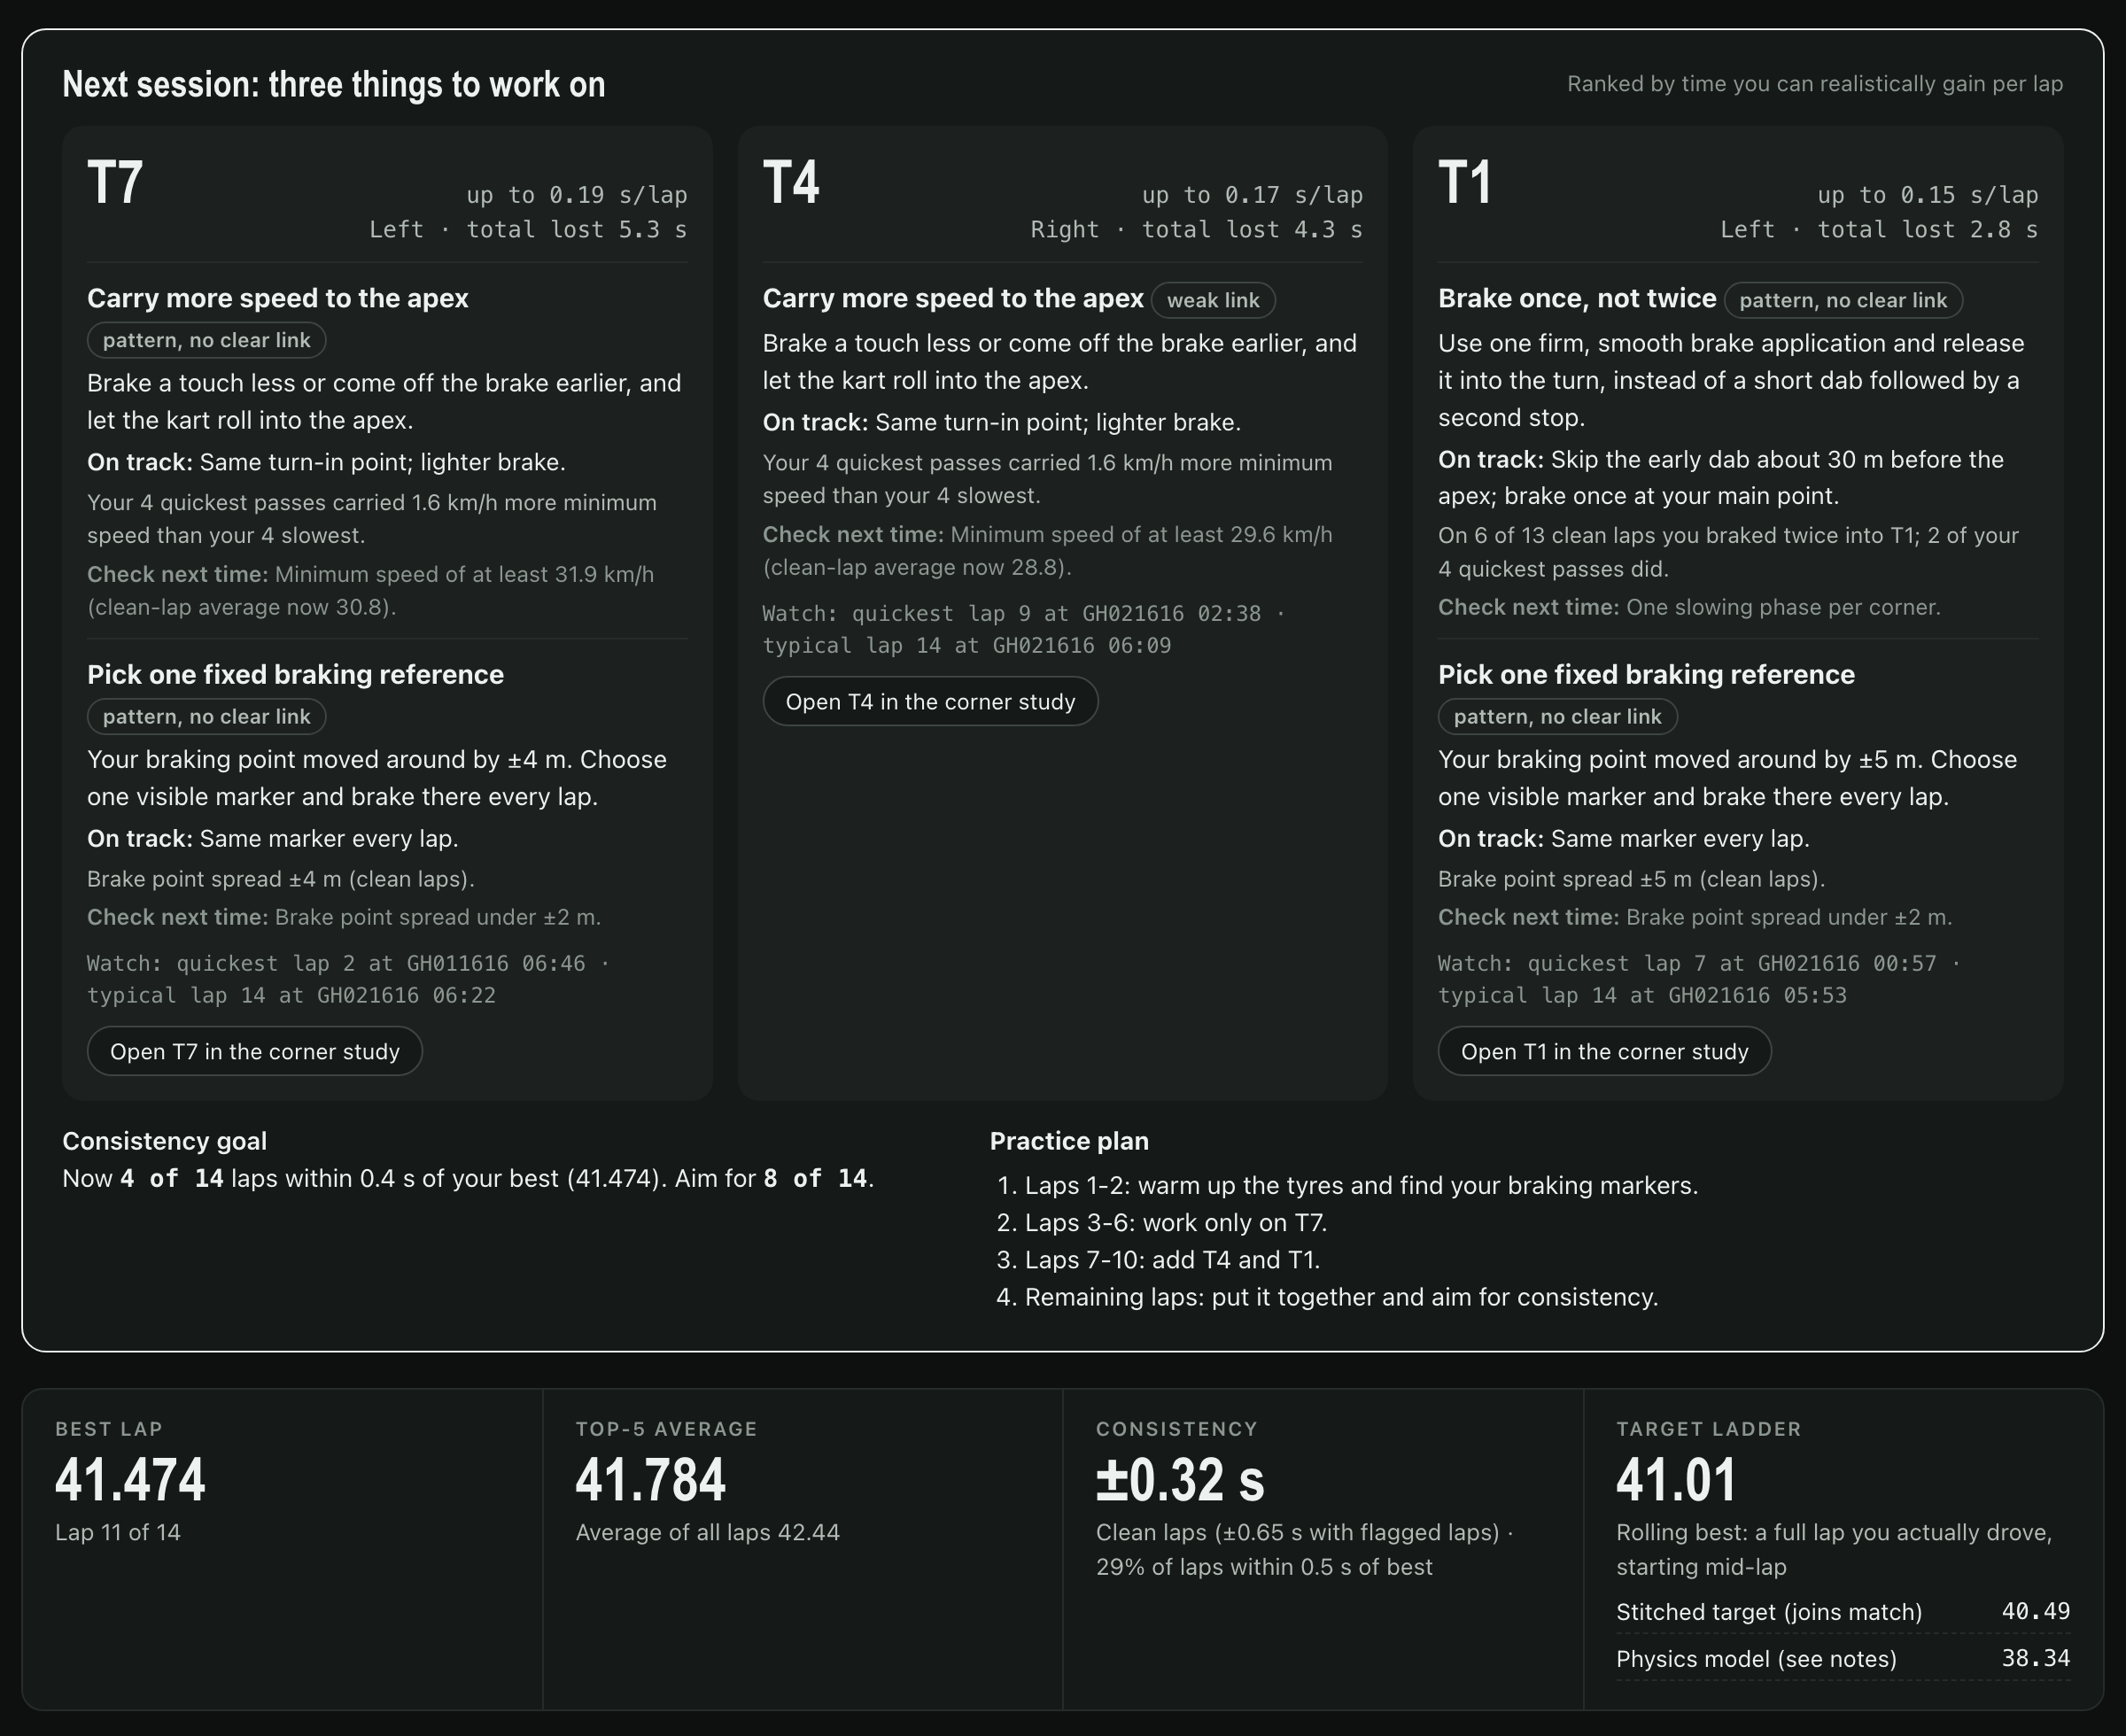
\includegraphics[width=\linewidth,height=0.82\textheight,keepaspectratio]{img/session-debrief.png}
    \end{column}
    \begin{column}{0.35\textwidth}
      \begin{itemize}
        \item Реальна сесія: 14 кіл, «Жага швидкості», GoPro HERO7
        \item Три повороти з порадами й планом на наступний заїзд
        \item Біля кожної поради — момент у відео
      \end{itemize}
    \end{column}
  \end{columns}

  \note{[Доповідач 4] Ось як це виглядатиме. Це макет розбору однієї реальної сесії: 14 кіл на картодромі «Жага швидкості», знято на GoPro HERO7. Угорі — блок «три речі, над якими працювати»: повороти, де можна виграти найбільше часу. Для кожного є порада простими словами і цифра, яку варто перевірити наступного разу, а також посилання на момент у відео. Нижче — план на наступний заїзд і підсумкові цифри сесії. У повному макеті є ще карта траси з межами і таблиця часу по колах. Саме такий результат пілот має отримувати після кожного заїзду.}
\end{frame}

% ===== 11. Ризики =====
\begin{frame}{Ризики і як ми з ними працюємо}
  \centering
  \begin{tabularx}{\textwidth}{@{}>{\raggedright\arraybackslash}p{0.38\textwidth} >{\raggedright\arraybackslash}X@{}}
    \toprule
    \textbf{Ризик зі SWOT} & \textbf{Що робимо в проєкті} \\
    \midrule
    Точність GPS у телефоні \textasciitilde{}4,9 м (W1)
      & Основне джерело — GoPro з GPS, телефон — з попередженням \\
    Точні межі траси потребують фото з дрона (W6)
      & Межі із супутника, невпевнені ділянки — пунктиром \\
    Криті картодроми без GPS (W3)
      & MVP — лише відкриті траси \\
    Tenth Finder і Kart Track уже дають поради (T1)
      & Перевіряємо їх до розробки; ми — без нового обладнання \\
    \bottomrule
  \end{tabularx}

  \note{[Доповідач 4] Звісно, ризики є, і ми їх не ховаємо. Точність GPS у телефоні — близько 4,9 метра. Тому основним джерелом буде відео GoPro з GPS, а трек із телефона підтримаємо з попередженням про точність. Точні межі траси потребують фото з дрона, тож у MVP беремо межі із супутникових знімків, а невпевнені ділянки показуємо пунктиром і порад щодо траєкторії там не даємо. Криті картодроми без GPS у MVP не входять. А конкурентів, Tenth Finder і Kart Track, ми встановимо й перевіримо ще до розробки. Повний список ризиків і рішень є в документі з рішенням.}
\end{frame}

% ===== 12. Наступні кроки =====
\begin{frame}{Наступні кроки}
  \begin{enumerate}
    \setlength{\itemsep}{6pt}
    \item \textbf{Обсяг MVP:} відео GoPro, одна відкрита траса, 2–3 поради
    \item \textbf{Технології:} перевірити gopro-telemetry
    \item \textbf{Методика демо:} що автоматизуємо — межі, зсув GPS
    \item \textbf{Супутникові знімки:} перевірити умови використання
    \item \textbf{Конкуренти:} встановити Tenth Finder і Kart Track
  \end{enumerate}

  \note{[Доповідач 4] Що далі. Спочатку визначаємо обсяг MVP: відео GoPro, одна відкрита траса, поділ на кола, втрати часу по поворотах і дві-три поради. Потім обираємо технології і першою перевіряємо бібліотеку gopro-telemetry. Також розбираємо методику нашого демо і вирішуємо, що з неї робимо автоматично: обведення меж траси за супутником і корекцію зсуву GPS. Окремо треба перевірити умови використання супутникових знімків. І ще до розробки встановлюємо Tenth Finder і Kart Track, щоб зрозуміти, яке обладнання їм потрібне і чим ми від них відрізняємося.}
\end{frame}

% ===== 13. Дякуємо =====
\begin{frame}[standout]
  Дякуємо за увагу!\\[0.3em]
  Запитання?

  \vspace{1.5em}
  \raggedright\footnotesize\mdseries
  Повний SWOT і джерела:\\
  \texttt{docs/stages/stage-1/lap-coach/SWOT.md}\\
  \texttt{docs/stages/stage-1/smart-grocery/SWOT.md}\\
  Рішення, критерії, ризики: \texttt{docs/stages/stage-1/Decision.md}\\
  Макет розбору заїзду: \texttt{docs/stages/stage-1/lap-coach/Karting-session.html}

  \note{[Доповідач 4] Дякуємо за увагу! Коротко ще раз: ми розглянули дві теми, описали їх, зробили SWOT-аналіз, порівняли за п'ятьма критеріями й обрали цифровий тренер для автоспорту. Він виграє за конкурентною перевагою і меншою залежністю від однієї компанії. Внизу слайда — шляхи до файлів із повним SWOT-аналізом, джерелами і документом з рішенням: там є всі цифри, які ми сьогодні називали, з посиланнями. Якщо цікаво, можемо відкрити макет розбору заїзду в браузері. Будемо раді вашим запитанням.}
\end{frame}


\end{document}

\ifdefined\shownotes
  \usepackage{pgfpages}
  \setbeameroption{show notes on second screen=right}
  % XeLaTeX + pgfpages: після кольорового тексту колір не відновлюється
  % (основний текст стає білим). Переводимо кольори на pdfcolorstack,
  % який після кожного pop явно повертає поточний колір.
  \makeatletter
  \def\nt@conv#1 #2\@nil{\csname nt@conv@#1\endcsname#2\@nil}
  \def\nt@conv@rgb#1 #2 #3\@nil{#1 #2 #3 rg #1 #2 #3 RG}
  \def\nt@conv@gray#1\@nil{#1 g #1 G}
  \def\nt@conv@cmyk#1 #2 #3 #4\@nil{#1 #2 #3 #4 k #1 #2 #3 #4 K}
  \AtBeginDocument{%
    \special{pdfcolorstackinit 1 page direct (0 g 0 G)}%
    \def\beamerorig@set@color{%
      \edef\nt@tmp{\current@color\space}%
      \special{pdfcolorstack 1 push (\expandafter\nt@conv\nt@tmp\@nil)}%
      \aftergroup\reset@color}%
    \def\beamerorig@reset@color{%
      \special{pdfcolorstack 1 pop}\special{pdfcolorstack 1 current}}%
  }
  \makeatother
\fi

% ---------- Тема ----------
\usetheme[progressbar=frametitle,numbering=counter]{metropolis}
\setbeamertemplate{navigation symbols}{}

% ---------- Кольори (усе в одному місці) ----------
\definecolor{accent}{HTML}{C8461B}   % акцент
\definecolor{ink}{HTML}{23272B}      % темний нейтральний
\colorlet{swotS}{accent}
\colorlet{swotO}{accent!70!black}
\colorlet{swotW}{ink}
\colorlet{swotT}{ink!60}
\colorlet{highlight}{accent!15}

\setbeamercolor{frametitle}{bg=ink,fg=white}
\setbeamercolor{progress bar}{fg=accent,bg=accent!20}
\setbeamercolor{title separator}{fg=accent}
\setbeamercolor{alerted text}{fg=accent}
\setbeamercolor{background canvas}{bg=white}
\setbeamercolor{normal text}{fg=ink}
\setbeamercolor{standout}{bg=ink,fg=white}
\setbeamercolor{itemize item}{fg=accent}
\setbeamercolor{enumerate item}{fg=accent}

% ---------- Мова і шрифти ----------
\usepackage{fontspec}
\usepackage{polyglossia}
\setdefaultlanguage{ukrainian}
\setotherlanguage{english}
% PT Sans з TeX Live (пакет paratype), підключений за іменами файлів
\defaultfontfeatures{Ligatures=TeX}
\setmainfont{PTS55F.ttf}[BoldFont=PTS75F.ttf,ItalicFont=PTS56F.ttf,BoldItalicFont=PTS76F.ttf]
\setsansfont{PTS55F.ttf}[BoldFont=PTS75F.ttf,ItalicFont=PTS56F.ttf,BoldItalicFont=PTS76F.ttf]
\newfontfamily\cyrillicfont{PTS55F.ttf}[BoldFont=PTS75F.ttf,ItalicFont=PTS56F.ttf,BoldItalicFont=PTS76F.ttf]
\newfontfamily\cyrillicfontsf{PTS55F.ttf}[BoldFont=PTS75F.ttf,ItalicFont=PTS56F.ttf,BoldItalicFont=PTS76F.ttf]
\setmonofont{PTM55F.ttf}[Scale=MatchLowercase]
\setbeamerfont{frametitle}{series=\bfseries}
\setbeamerfont{title}{series=\bfseries}

% ---------- Пакети ----------
\usepackage{booktabs}
\usepackage{array}
\usepackage{tabularx}
\usepackage{graphicx}
\usepackage{tikz}
\usetikzlibrary{positioning,arrows.meta}
\usepackage[most]{tcolorbox}

\renewcommand{\arraystretch}{1.25}

% SWOT-квадрант: #1 колір, #2 літера, #3 підпис, #4 пункти, #5 група рівної висоти
\newcommand{\swotbox}[5]{%
  \begin{tcolorbox}[enhanced,colframe=#1,colback=#1!7,boxrule=0.6pt,arc=2pt,
    equal height group=#5,left=4pt,right=4pt,top=2pt,bottom=2pt,
    fonttitle=\bfseries\small,coltitle=white,colbacktitle=#1,
    toptitle=1pt,bottomtitle=1pt,
    title={\large #2\enspace\normalsize\mdseries #3}]
    \small\setlength{\leftmargini}{1.1em}
    \begin{itemize}\setlength{\itemsep}{1pt}
      #4
    \end{itemize}
  \end{tcolorbox}}

\newcommand{\swotgrid}[4]{%
  \begin{columns}[T,onlytextwidth]
    \begin{column}{0.49\textwidth}
      \swotbox{swotS}{S}{Сильні сторони}{#1}{swottop}\vspace{-4pt}
      \swotbox{swotO}{O}{Можливості}{#3}{swotbottom}
    \end{column}
    \begin{column}{0.49\textwidth}
      \swotbox{swotW}{W}{Слабкі сторони}{#2}{swottop}\vspace{-4pt}
      \swotbox{swotT}{T}{Загрози}{#4}{swotbottom}
    \end{column}
  \end{columns}}

% ---------- Титульні дані ----------
\title{Вибір теми командного проєкту}
\subtitle{Обрана тема: «Цифровий тренер для автоспорту»}
\date{}

\begin{document}

% ===== 1. Титульний =====
\begin{frame}[plain]
  \vspace*{-0.6cm}\titlepage
  \note{[Доповідач 1] Добрий день! Ми сьогодні захищаємо перший етап командного проєкту — вибір теми. Одразу скажемо результат: ми обрали тему «Цифровий тренер для автоспорту». Це вебзастосунок, який перетворює GPS-запис з екшн-камери чи телефона на розбір заїзду з порадами. Але до цього рішення ми дійшли не одразу. Ми розглянули дві ідеї, для кожної написали опис і зробили SWOT-аналіз, а потім порівняли їх за однаковими критеріями. Далі покажемо весь цей шлях по кроках. Говоритимемо по черзі, кожен про свою частину.}
\end{frame}

% ===== 2. Мета і процес =====
\begin{frame}{Мета етапу і як ми обирали тему}
  \textbf{Мета:} обрати тему командного проєкту й обґрунтувати вибір.

  \vspace{1.2em}
  \centering
  \begin{tikzpicture}[
      stp/.style={draw=accent,fill=accent!8,rounded corners=3pt,line width=0.8pt,
        minimum width=2.15cm,minimum height=1.1cm,align=center,font=\small\bfseries},
      final/.style={stp,fill=accent,text=white},
      desc/.style={font=\small,text width=2.3cm,align=center,text=ink!80},
      arr/.style={-{Stealth[length=2.2mm]},line width=0.9pt,draw=ink!60},
      node distance=0.5cm]
    \node[stp] (s1) {Ідеї};
    \node[stp,right=of s1] (s2) {Опис};
    \node[stp,right=of s2] (s3) {SWOT};
    \node[stp,right=of s3] (s4) {Порівняння\\за критеріями};
    \node[final,right=of s4] (s5) {Рішення};
    \foreach \a/\b in {s1/s2,s2/s3,s3/s4,s4/s5} \draw[arr] (\a) -- (\b);
    \node[desc,below=0.3cm of s1] {дві теми};
    \node[desc,below=0.3cm of s2] {що, для кого, яка проблема};
    \node[desc,below=0.3cm of s3] {сильні й слабкі сторони, можливості, загрози};
    \node[desc,below=0.3cm of s4] {5 критеріїв з вагами, оцінки 1–5};
    \node[desc,below=0.3cm of s5] {цифровий тренер для автоспорту};
  \end{tikzpicture}

  \note{[Доповідач 1] Мета етапу — не просто назвати тему, а обґрунтувати, чому саме її. Тому ми йшли за простою схемою з п'яти кроків. Спочатку зібрали ідеї: у підсумку їх дві — цифровий тренер для автоспорту і розумний кошик для товарів. Для кожної написали опис: що це, для кого і яку проблему вирішує. Потім зробили SWOT-аналіз із джерелами. Далі домовилися про п'ять критеріїв з вагами і поставили кожній темі оцінки від одного до п'яти. І лише після цього ухвалили рішення. Так обидві теми ми порівнювали за однаковими правилами, а не за враженням.}
\end{frame}

% ===== 3. Тема 1 =====
\begin{frame}{Тема 1. Цифровий тренер для автоспорту}
  \begin{columns}[T,onlytextwidth]
    \begin{column}{0.48\textwidth}
      \textbf{\color{accent}Призначення}\\
      Вебзастосунок: GPS-запис з камери чи телефона $\to$ розбір заїзду

      \medskip
      \textbf{\color{accent}Для кого}\\
      Новачки й аматори без тренера: прокатний картинг, трек-дні

      \medskip
      \textbf{\color{accent}Проблема}\\
      Немає об'єктивного зворотного зв'язку, тренер і телеметрія дорогі
    \end{column}
    \begin{column}{0.48\textwidth}
      \textbf{\color{accent}Основні можливості}
      \begin{itemize}
        \item Автоматичний поділ заїзду на кола
        \item Траєкторія на карті траси з межами
        \item Повороти, де втрачається найбільше часу
        \item 2–3 поради простою мовою з відео
      \end{itemize}
    \end{column}
  \end{columns}

  \note{[Доповідач 1] Перша тема — цифровий тренер для автоспорту. Уявіть новачка, який регулярно їздить на прокатний картинг. Він відчуває, що десь втрачає час, але не знає, де саме і що змінити. Живий тренер дорогий, а професійна телеметрія розрахована на досвідчених пілотів. Наш застосунок бере запис з екшн-камери GoPro чи трек із телефона, сам ділить заїзд на кола, накладає траєкторію на реальні межі траси і знаходить повороти, де пілот втрачає найбільше часу. На виході — не графіки, а дві-три поради простою мовою з цифрами і фрагментом відео, плюс план на наступний заїзд.}
\end{frame}

% ===== 4. Тема 2 =====
\begin{frame}{Тема 2. Розумний кошик для товарів}
  \begin{columns}[T,onlytextwidth]
    \begin{column}{0.48\textwidth}
      \textbf{\color{accent}Призначення}\\
      Окремий застосунок сам складає кошик у Сільпо через MCP

      \medskip
      \textbf{\color{accent}Для кого}\\
      Зайняті люди 22–40 років у великих містах, клієнти Сільпо

      \medskip
      \textbf{\color{accent}Проблема}\\
      Планувати їжу й покупки щодня — рутина, продукти викидають
    \end{column}
    \begin{column}{0.48\textwidth}
      \textbf{\color{accent}Основні можливості}
      \begin{itemize}
        \item Оцінка того, що є вдома, за історією покупок
        \item План харчування на 2–3 дні
        \item Автоматичний кошик із поясненнями
        \item Підтвердження, доставка чи самовивіз
      \end{itemize}
    \end{column}
  \end{columns}

  \note{[Доповідач 2] Друга тема — розумний кошик для товарів. Ідея така: застосунок сам складає замовлення в Сільпо на найближчі дні. Він знає, що людина зазвичай купує, за історією покупок оцінює, що вже закінчилося вдома, і пропонує простий план харчування на два-три дні. Увечері людина отримує готовий кошик, де біля кожного товару написана причина. Їй лишається переглянути його і обрати доставку чи самовивіз. Працює це через офіційний MCP-сервер, який Сільпо відкрило в серпні 2026 року. Аудиторія — зайняті люди 22–40 років у великих містах, які вже купують у Сільпо.}
\end{frame}

% ===== 5. SWOT: цифровий тренер =====
\begin{frame}{SWOT: цифровий тренер для автоспорту}
  \swotgrid
    {\item Не потрібне нове обладнання
     \item Відкритий формат GPMF і бібліотеки
     \item Демо: середня похибка кола 0,035 с}
    {\item GPS у телефоні: точність \textasciitilde{}4,9 м
     \item Криті картодроми без GPS
     \item Межі траси з відео поки не будуються}
    {\item Живий тренер — €250–350 на день
     \item Track Titan: 200\,000+ користувачів
     \item Ріст картингу: K1 Speed — 107 локацій}
    {\item Tenth Finder і Kart Track дають поради
     \item Дешевий RaceChrono Pro за \$19.99
     \item Камери без GPS, як HERO12}

  \note{[Доповідач 2] Тепер SWOT цифрового тренера. Головна сила — пілоту не треба купувати нове обладнання, досить камери чи телефона. GoPro зберігає телеметрію у відкритому форматі GPMF, і для нього вже є бібліотеки. А наше демо на реальній сесії показало, що час кола за GPS відрізняється від офіційного хронометражу в середньому на 0,035 секунди. Слабкі місця — точність GPS у телефоні, криті картодроми без сигналу і межі траси, які з відео поки не будуються. Можливості — дорогі живі тренери й інвестиції в Track Titan. Загрози — конкуренти, які вже дають поради, дешевий RaceChrono і те, що Камери без GPS, як HERO12.}
\end{frame}

% ===== 6. SWOT: розумний кошик =====
\begin{frame}{SWOT: розумний кошик для товарів}
  \swotgrid
    {\item Офіційний MCP: 40 інструментів
     \item Історія покупок онлайн і в магазинах
     \item Сам пропонує кошик, не чекає запиту}
    {\item «Що є вдома» — лише здогадка
     \item Кошик помиляється з фасуваннями
     \item Усі дані належать Сільпо}
    {\item 81\% купують продукти в магазинах
     \item Вибір страв: десятки хв на тиждень
     \item Відходи: 79 кг їжі на людину на рік}
    {\item Сільпо може зробити те саме
     \item Залежність від правил одного MCP
     \item Харчові дані можуть бути чутливими}

  \note{[Доповідач 2] SWOT розумного кошика. Сильна сторона — офіційний доступ до Сільпо: сорок інструментів, вхід через OAuth і приклади коду. До того ж видно історію покупок не лише онлайн, а й у магазинах. І продукт сам приходить з кошиком, а не чекає запиту. Але оцінка того, що є вдома, — лише здогадка, а в тестах автоматичний кошик уже помилявся з фасуваннями й наявністю. Власних даних у нас немає. Можливості — 81\% українців досі купують продукти в магазинах, тож онлайну є куди рости, плюс тема харчових відходів. Головні загрози — Сільпо може зробити те саме у своєму застосунку, а ми повністю залежимо від правил одного сервера.}
\end{frame}

% ===== 7. Критерії і ваги =====
\begin{frame}{Критерії і ваги}
  \centering
  \begin{tabular}{@{}l c l@{}}
    \toprule
    \textbf{Критерій} & \textbf{Вага} & \textbf{Що означає} \\
    \midrule
    Актуальність проблеми        & 0,25 & Наскільки проблема важлива для аудиторії \\
    Реалізованість за семестр    & 0,25 & Чи зробимо робочий продукт \\
    Конкурентна перевага         & 0,2  & Чим ми кращі за наявні рішення \\
    Інтерес і досвід команди     & 0,15 & Чи хочемо і чи маємо потрібні знання \\
    Ризики і зовнішні залежності & 0,15 & Менше ризиків — вища оцінка \\
    \midrule
    \textbf{Разом}               & \textbf{1,0} & \\
    \bottomrule
  \end{tabular}

  \note{[Доповідач 3] Щоб порівняти теми чесно, ми домовилися про п'ять критеріїв. Найбільшу вагу, по 0,25, мають актуальність проблеми і реалізованість за семестр. Тобто продукт має бути потрібним, і ми маємо встигнути його зробити. Конкурентна перевага важить 0,2: чим ми кращі за те, що вже є. Інтерес і досвід команди та ризики — по 0,15. Для ризиків шкала обернена: що менше ризиків і зовнішніх залежностей, то вища оцінка. Разом ваги дають одиницю, тож підсумок — це зважена оцінка на тій самій шкалі від одного до п'яти.}
\end{frame}

% ===== 8. Порівняння =====
\begin{frame}{Порівняння тем}
  \centering\renewcommand{\arraystretch}{1.1}
  \begin{tabular}{@{}l c >{\columncolor{highlight}}c c@{}}
    \toprule
    \textbf{Критерій} & \textbf{Вага} & \textbf{\begin{tabular}{@{}c@{}}Цифровий\\тренер\end{tabular}} & \textbf{\begin{tabular}{@{}c@{}}Розумний\\кошик\end{tabular}} \\
    \midrule
    Актуальність проблеми        & 0,25 & 4 & 4 \\
    Реалізованість за семестр    & 0,25 & 4 & 4 \\
    Конкурентна перевага         & 0,2  & 3 & 2 \\
    Інтерес і досвід команди     & 0,15 & ? & ? \\
    Ризики і зовнішні залежності & 0,15 & 3 & 2 \\
    \midrule
    \textbf{Зважена сума без «інтересу»} (макс. 4,25) & 0,85 & \textbf{3,05} & \textbf{2,70} \\
    \bottomrule
  \end{tabular}

  \vspace{0.3em}
  \raggedright\small
  Підсумок = зважена сума + 0,15 × середня оцінка інтересу команди.\\
  Кошик випередить тренера, лише якщо його інтерес вищий хоча б на 3 бали.

  \note{[Доповідач 3] Ось самі оцінки. За актуальністю і реалізованістю теми рівні — обидві по 4. Різниця з'являється в конкурентній перевазі: 3 у тренера проти 2 у кошика. І в ризиках теж 3 проти 2. Оцінки за інтерес команди ми ще не зібрали, тому там знаки питання, і зважену суму рахуємо без цього критерію: максимум тут 4,25. Тренер має 3,05, кошик — 2,70, різниця 0,35 бала. Коли кожен з нас поставить свою оцінку, ми додамо 0,15, помножене на середнє. Кошик виграв би, лише якби ми оцінили його інтерес хоча б на 3 бали вище.}
\end{frame}

% ===== 9. Чому цифровий тренер =====
\newcommand{\argcard}[2]{%
  \begin{tcolorbox}[colframe=accent,colback=accent!6,boxrule=0.6pt,arc=2pt,
    height=2.55cm,valign=top,left=5pt,right=5pt,top=4pt,bottom=4pt]
    \raggedright\textbf{#1}\par\smallskip
    \small #2
  \end{tcolorbox}}

\begin{frame}{Чому цифровий тренер}
  \begin{columns}[T,onlytextwidth]
    \begin{column}{0.49\textwidth}
      \argcard{Працює з тим, що в пілота вже є}
        {Камера чи телефон, а не Garmin Catalyst 2 за \$1,199.99}
      \argcard{Люди готові платити за тренування}
        {Живий тренер — €250–350 на день, Track Titan залучив \$5 млн}
    \end{column}
    \begin{column}{0.49\textwidth}
      \argcard{Дані відкриті й належать пілоту}
        {Формат GPMF у відеофайлі, без API чи дозволу компаній}
      \argcard{Поради, а не графіки}
        {2–3 поради з цифрами й відео для новачка}
    \end{column}
  \end{columns}

  \note{[Доповідач 3] Чому саме цифровий тренер? Перше: він працює з тим, що в пілота вже є, — з камерою чи телефоном, а не з пристроєм на кшталт Garmin Catalyst 2 за \$1,199.99. Друге: дані відкриті. GoPro пише телеметрію у форматі GPMF прямо у відеофайл, і цей файл належить пілоту. Нам не потрібен дозвіл чи API жодної компанії — на відміну від кошика. Третє: люди вже платять за тренування. Живий тренер коштує €250–350 на день, а Track Titan залучив \$5 млн. І четверте: ми закриваємо проміжок між графіками і дорогими пристроями — даємо новачку дві-три поради з цифрами і відео.}
\end{frame}

% ===== 10. Як виглядатиме продукт =====
\begin{frame}{Як виглядатиме продукт}
  \begin{columns}[c,onlytextwidth]
    \begin{column}{0.62\textwidth}
      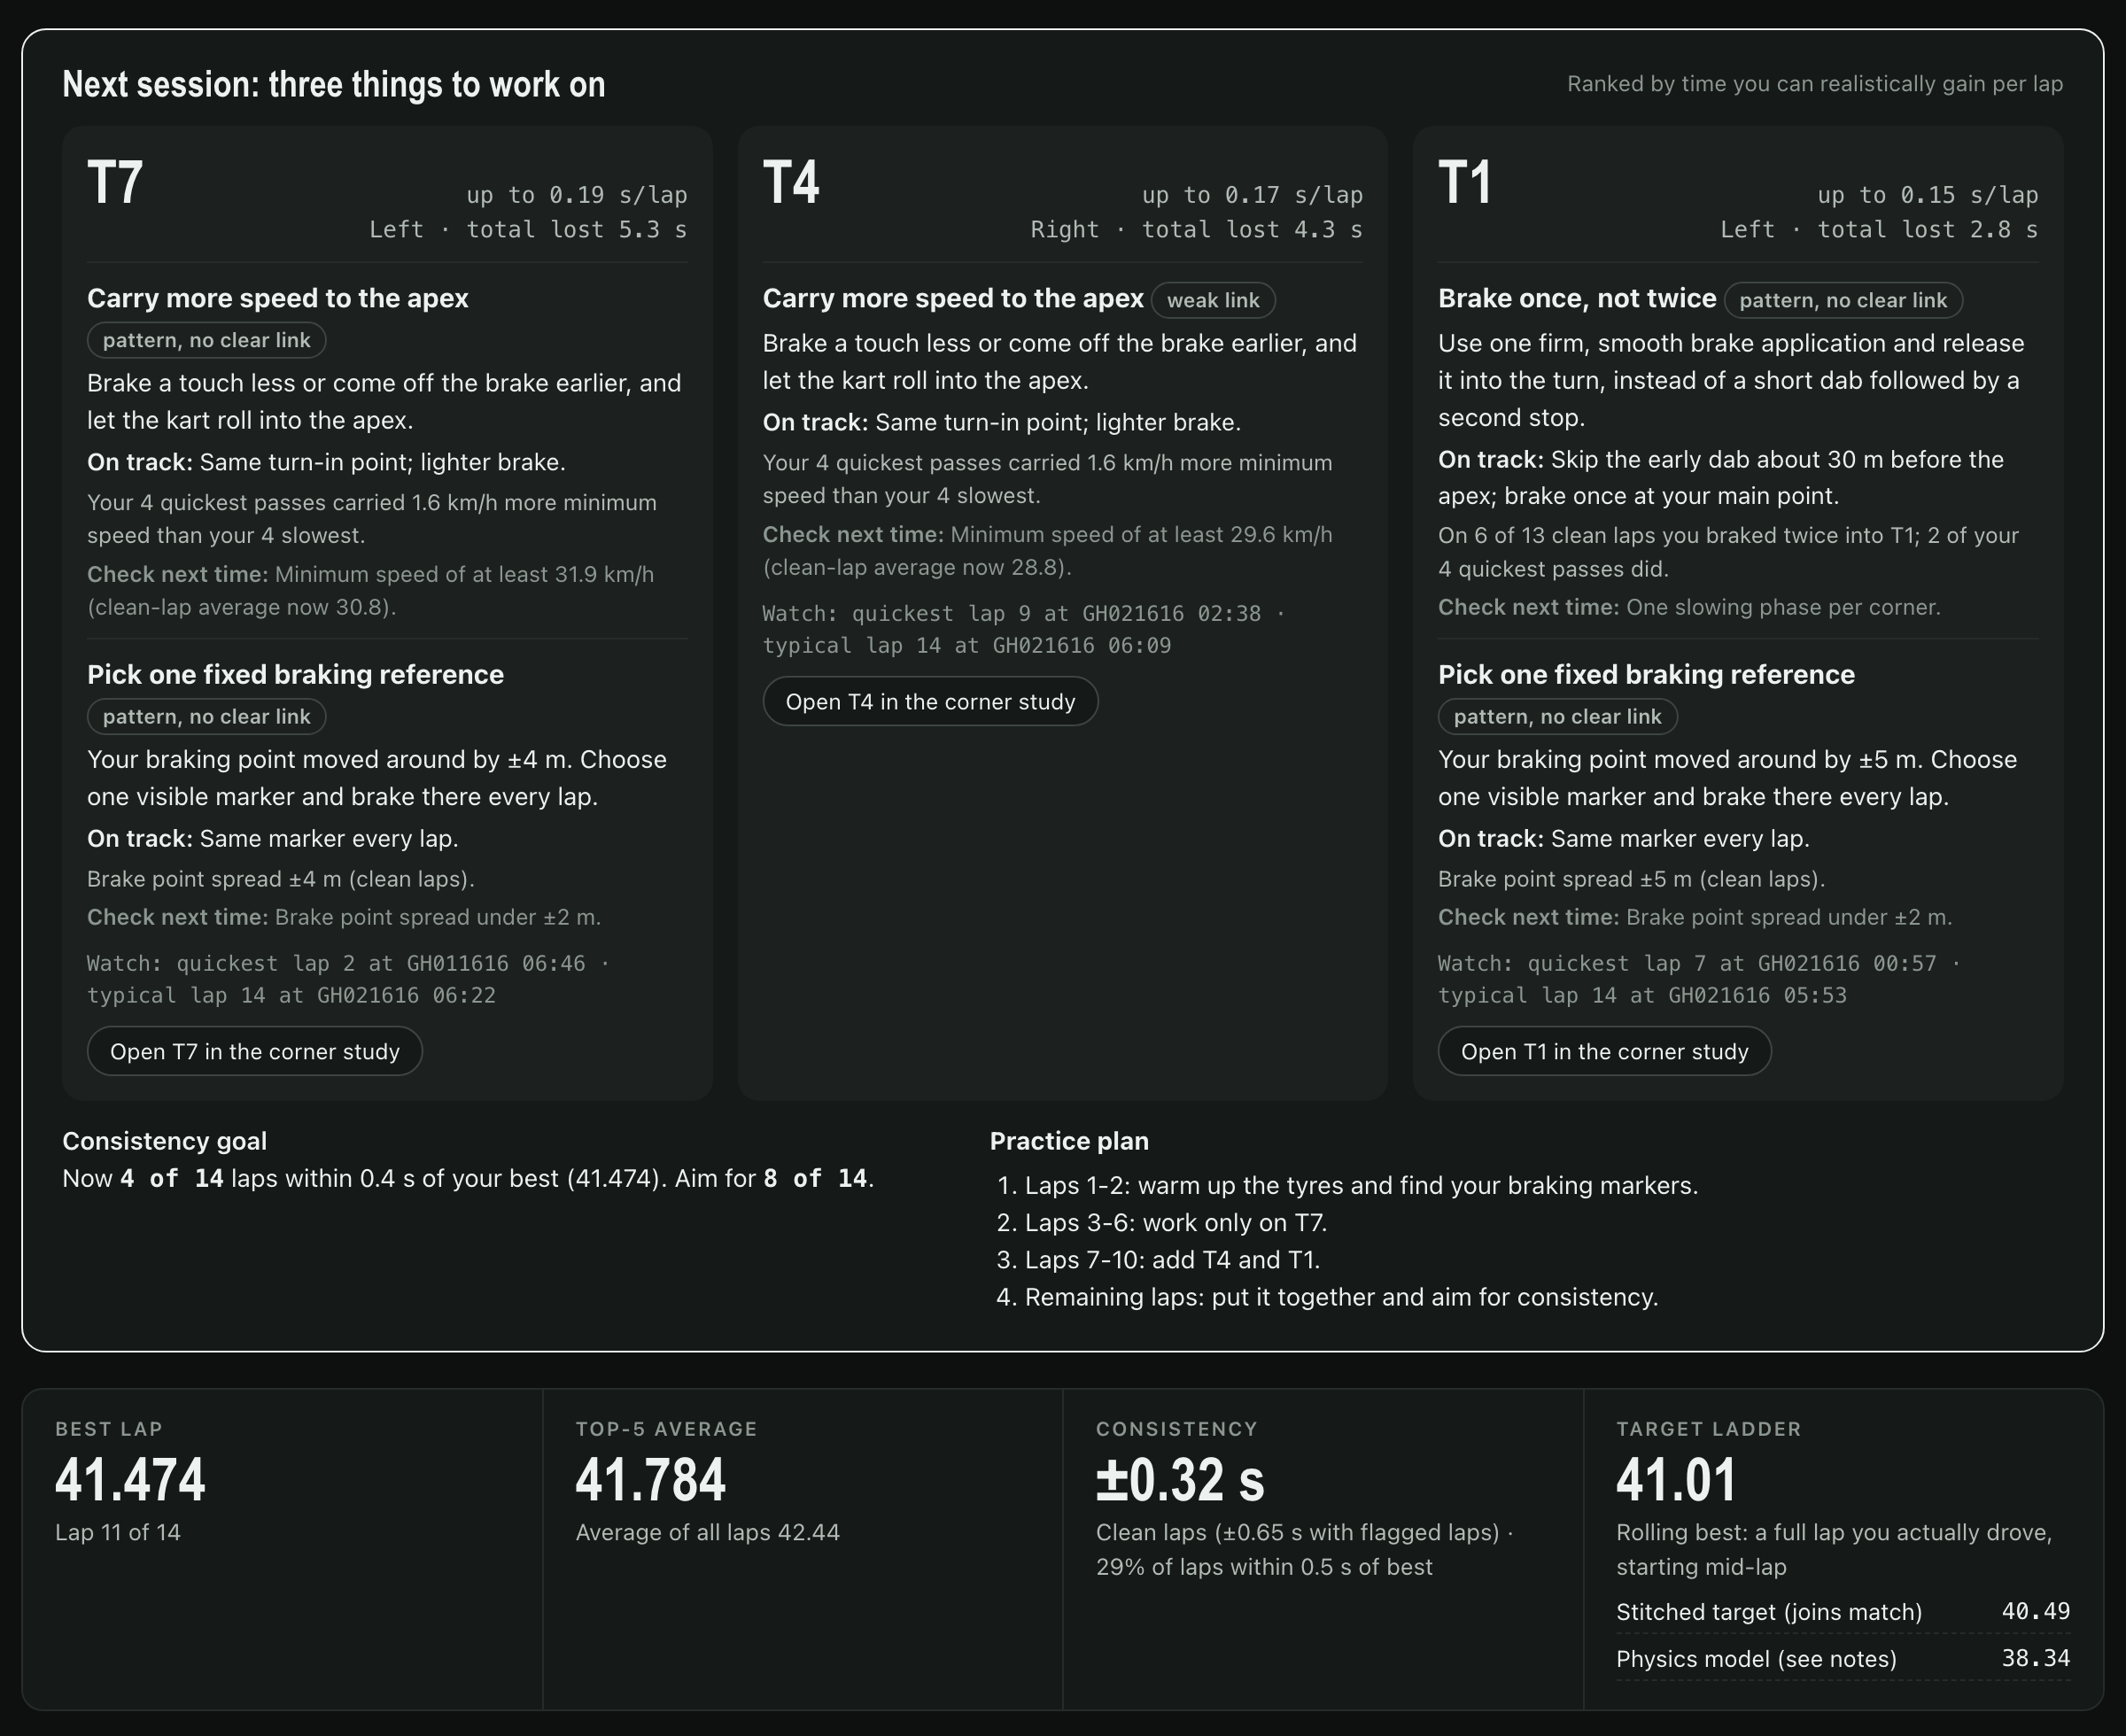
\includegraphics[width=\linewidth,height=0.82\textheight,keepaspectratio]{img/session-debrief.png}
    \end{column}
    \begin{column}{0.35\textwidth}
      \begin{itemize}
        \item Реальна сесія: 14 кіл, «Жага швидкості», GoPro HERO7
        \item Три повороти з порадами й планом на наступний заїзд
        \item Біля кожної поради — момент у відео
      \end{itemize}
    \end{column}
  \end{columns}

  \note{[Доповідач 4] Ось як це виглядатиме. Це макет розбору однієї реальної сесії: 14 кіл на картодромі «Жага швидкості», знято на GoPro HERO7. Угорі — блок «три речі, над якими працювати»: повороти, де можна виграти найбільше часу. Для кожного є порада простими словами і цифра, яку варто перевірити наступного разу, а також посилання на момент у відео. Нижче — план на наступний заїзд і підсумкові цифри сесії. У повному макеті є ще карта траси з межами і таблиця часу по колах. Саме такий результат пілот має отримувати після кожного заїзду.}
\end{frame}

% ===== 11. Ризики =====
\begin{frame}{Ризики і як ми з ними працюємо}
  \centering
  \begin{tabularx}{\textwidth}{@{}>{\raggedright\arraybackslash}p{0.38\textwidth} >{\raggedright\arraybackslash}X@{}}
    \toprule
    \textbf{Ризик зі SWOT} & \textbf{Що робимо в проєкті} \\
    \midrule
    Точність GPS у телефоні \textasciitilde{}4,9 м (W1)
      & Основне джерело — GoPro з GPS, телефон — з попередженням \\
    Точні межі траси потребують фото з дрона (W6)
      & Межі із супутника, невпевнені ділянки — пунктиром \\
    Криті картодроми без GPS (W3)
      & MVP — лише відкриті траси \\
    Tenth Finder і Kart Track уже дають поради (T1)
      & Перевіряємо їх до розробки; ми — без нового обладнання \\
    \bottomrule
  \end{tabularx}

  \note{[Доповідач 4] Звісно, ризики є, і ми їх не ховаємо. Точність GPS у телефоні — близько 4,9 метра. Тому основним джерелом буде відео GoPro з GPS, а трек із телефона підтримаємо з попередженням про точність. Точні межі траси потребують фото з дрона, тож у MVP беремо межі із супутникових знімків, а невпевнені ділянки показуємо пунктиром і порад щодо траєкторії там не даємо. Криті картодроми без GPS у MVP не входять. А конкурентів, Tenth Finder і Kart Track, ми встановимо й перевіримо ще до розробки. Повний список ризиків і рішень є в документі з рішенням.}
\end{frame}

% ===== 12. Наступні кроки =====
\begin{frame}{Наступні кроки}
  \begin{enumerate}
    \setlength{\itemsep}{6pt}
    \item \textbf{Обсяг MVP:} відео GoPro, одна відкрита траса, 2–3 поради
    \item \textbf{Технології:} перевірити gopro-telemetry
    \item \textbf{Методика демо:} що автоматизуємо — межі, зсув GPS
    \item \textbf{Супутникові знімки:} перевірити умови використання
    \item \textbf{Конкуренти:} встановити Tenth Finder і Kart Track
  \end{enumerate}

  \note{[Доповідач 4] Що далі. Спочатку визначаємо обсяг MVP: відео GoPro, одна відкрита траса, поділ на кола, втрати часу по поворотах і дві-три поради. Потім обираємо технології і першою перевіряємо бібліотеку gopro-telemetry. Також розбираємо методику нашого демо і вирішуємо, що з неї робимо автоматично: обведення меж траси за супутником і корекцію зсуву GPS. Окремо треба перевірити умови використання супутникових знімків. І ще до розробки встановлюємо Tenth Finder і Kart Track, щоб зрозуміти, яке обладнання їм потрібне і чим ми від них відрізняємося.}
\end{frame}

% ===== 13. Дякуємо =====
\begin{frame}[standout]
  Дякуємо за увагу!\\[0.3em]
  Запитання?

  \vspace{1.5em}
  \raggedright\footnotesize\mdseries
  Повний SWOT і джерела:\\
  \texttt{docs/stages/stage-1/lap-coach/SWOT.md}\\
  \texttt{docs/stages/stage-1/smart-grocery/SWOT.md}\\
  Рішення, критерії, ризики: \texttt{docs/stages/stage-1/Decision.md}\\
  Макет розбору заїзду: \texttt{docs/stages/stage-1/lap-coach/Karting-session.html}

  \note{[Доповідач 4] Дякуємо за увагу! Коротко ще раз: ми розглянули дві теми, описали їх, зробили SWOT-аналіз, порівняли за п'ятьма критеріями й обрали цифровий тренер для автоспорту. Він виграє за конкурентною перевагою і меншою залежністю від однієї компанії. Внизу слайда — шляхи до файлів із повним SWOT-аналізом, джерелами і документом з рішенням: там є всі цифри, які ми сьогодні називали, з посиланнями. Якщо цікаво, можемо відкрити макет розбору заїзду в браузері. Будемо раді вашим запитанням.}
\end{frame}


\end{document}

\ifdefined\shownotes
  \usepackage{pgfpages}
  \setbeameroption{show notes on second screen=right}
  % XeLaTeX + pgfpages: після кольорового тексту колір не відновлюється
  % (основний текст стає білим). Переводимо кольори на pdfcolorstack,
  % який після кожного pop явно повертає поточний колір.
  \makeatletter
  \def\nt@conv#1 #2\@nil{\csname nt@conv@#1\endcsname#2\@nil}
  \def\nt@conv@rgb#1 #2 #3\@nil{#1 #2 #3 rg #1 #2 #3 RG}
  \def\nt@conv@gray#1\@nil{#1 g #1 G}
  \def\nt@conv@cmyk#1 #2 #3 #4\@nil{#1 #2 #3 #4 k #1 #2 #3 #4 K}
  \AtBeginDocument{%
    \special{pdfcolorstackinit 1 page direct (0 g 0 G)}%
    \def\beamerorig@set@color{%
      \edef\nt@tmp{\current@color\space}%
      \special{pdfcolorstack 1 push (\expandafter\nt@conv\nt@tmp\@nil)}%
      \aftergroup\reset@color}%
    \def\beamerorig@reset@color{%
      \special{pdfcolorstack 1 pop}\special{pdfcolorstack 1 current}}%
  }
  \makeatother
\fi

% ---------- Тема ----------
\usetheme[progressbar=frametitle,numbering=counter]{metropolis}
\setbeamertemplate{navigation symbols}{}

% ---------- Кольори (усе в одному місці) ----------
\definecolor{accent}{HTML}{C8461B}   % акцент
\definecolor{ink}{HTML}{23272B}      % темний нейтральний
\colorlet{swotS}{accent}
\colorlet{swotO}{accent!70!black}
\colorlet{swotW}{ink}
\colorlet{swotT}{ink!60}
\colorlet{highlight}{accent!15}

\setbeamercolor{frametitle}{bg=ink,fg=white}
\setbeamercolor{progress bar}{fg=accent,bg=accent!20}
\setbeamercolor{title separator}{fg=accent}
\setbeamercolor{alerted text}{fg=accent}
\setbeamercolor{background canvas}{bg=white}
\setbeamercolor{normal text}{fg=ink}
\setbeamercolor{standout}{bg=ink,fg=white}
\setbeamercolor{itemize item}{fg=accent}
\setbeamercolor{enumerate item}{fg=accent}

% ---------- Мова і шрифти ----------
\usepackage{fontspec}
\usepackage{polyglossia}
\setdefaultlanguage{ukrainian}
\setotherlanguage{english}
% PT Sans з TeX Live (пакет paratype), підключений за іменами файлів
\defaultfontfeatures{Ligatures=TeX}
\setmainfont{PTS55F.ttf}[BoldFont=PTS75F.ttf,ItalicFont=PTS56F.ttf,BoldItalicFont=PTS76F.ttf]
\setsansfont{PTS55F.ttf}[BoldFont=PTS75F.ttf,ItalicFont=PTS56F.ttf,BoldItalicFont=PTS76F.ttf]
\newfontfamily\cyrillicfont{PTS55F.ttf}[BoldFont=PTS75F.ttf,ItalicFont=PTS56F.ttf,BoldItalicFont=PTS76F.ttf]
\newfontfamily\cyrillicfontsf{PTS55F.ttf}[BoldFont=PTS75F.ttf,ItalicFont=PTS56F.ttf,BoldItalicFont=PTS76F.ttf]
\setmonofont{PTM55F.ttf}[Scale=MatchLowercase]
\setbeamerfont{frametitle}{series=\bfseries}
\setbeamerfont{title}{series=\bfseries}

% ---------- Пакети ----------
\usepackage{booktabs}
\usepackage{array}
\usepackage{tabularx}
\usepackage{graphicx}
\usepackage{tikz}
\usetikzlibrary{positioning,arrows.meta}
\usepackage[most]{tcolorbox}

\renewcommand{\arraystretch}{1.25}

% SWOT-квадрант: #1 колір, #2 літера, #3 підпис, #4 пункти, #5 група рівної висоти
\newcommand{\swotbox}[5]{%
  \begin{tcolorbox}[enhanced,colframe=#1,colback=#1!7,boxrule=0.6pt,arc=2pt,
    equal height group=#5,left=4pt,right=4pt,top=2pt,bottom=2pt,
    fonttitle=\bfseries\small,coltitle=white,colbacktitle=#1,
    toptitle=1pt,bottomtitle=1pt,
    title={\large #2\enspace\normalsize\mdseries #3}]
    \small\setlength{\leftmargini}{1.1em}
    \begin{itemize}\setlength{\itemsep}{1pt}
      #4
    \end{itemize}
  \end{tcolorbox}}

\newcommand{\swotgrid}[4]{%
  \begin{columns}[T,onlytextwidth]
    \begin{column}{0.49\textwidth}
      \swotbox{swotS}{S}{Сильні сторони}{#1}{swottop}\vspace{-4pt}
      \swotbox{swotO}{O}{Можливості}{#3}{swotbottom}
    \end{column}
    \begin{column}{0.49\textwidth}
      \swotbox{swotW}{W}{Слабкі сторони}{#2}{swottop}\vspace{-4pt}
      \swotbox{swotT}{T}{Загрози}{#4}{swotbottom}
    \end{column}
  \end{columns}}

% ---------- Титульні дані ----------
\title{Вибір теми командного проєкту}
\subtitle{Обрана тема: «Цифровий тренер для автоспорту»}
\date{}

\begin{document}

% ===== 1. Титульний =====
\begin{frame}[plain]
  \vspace*{-0.6cm}\titlepage
  \note{[Доповідач 1] Добрий день! Ми сьогодні захищаємо перший етап командного проєкту — вибір теми. Одразу скажемо результат: ми обрали тему «Цифровий тренер для автоспорту». Це вебзастосунок, який перетворює GPS-запис з екшн-камери чи телефона на розбір заїзду з порадами. Але до цього рішення ми дійшли не одразу. Ми розглянули дві ідеї, для кожної написали опис і зробили SWOT-аналіз, а потім порівняли їх за однаковими критеріями. Далі покажемо весь цей шлях по кроках. Говоритимемо по черзі, кожен про свою частину.}
\end{frame}

% ===== 2. Мета і процес =====
\begin{frame}{Мета етапу і як ми обирали тему}
  \textbf{Мета:} обрати тему командного проєкту й обґрунтувати вибір.

  \vspace{1.2em}
  \centering
  \begin{tikzpicture}[
      stp/.style={draw=accent,fill=accent!8,rounded corners=3pt,line width=0.8pt,
        minimum width=2.15cm,minimum height=1.1cm,align=center,font=\small\bfseries},
      final/.style={stp,fill=accent,text=white},
      desc/.style={font=\small,text width=2.3cm,align=center,text=ink!80},
      arr/.style={-{Stealth[length=2.2mm]},line width=0.9pt,draw=ink!60},
      node distance=0.5cm]
    \node[stp] (s1) {Ідеї};
    \node[stp,right=of s1] (s2) {Опис};
    \node[stp,right=of s2] (s3) {SWOT};
    \node[stp,right=of s3] (s4) {Порівняння\\за критеріями};
    \node[final,right=of s4] (s5) {Рішення};
    \foreach \a/\b in {s1/s2,s2/s3,s3/s4,s4/s5} \draw[arr] (\a) -- (\b);
    \node[desc,below=0.3cm of s1] {дві теми};
    \node[desc,below=0.3cm of s2] {що, для кого, яка проблема};
    \node[desc,below=0.3cm of s3] {сильні й слабкі сторони, можливості, загрози};
    \node[desc,below=0.3cm of s4] {5 критеріїв з вагами, оцінки 1–5};
    \node[desc,below=0.3cm of s5] {цифровий тренер для автоспорту};
  \end{tikzpicture}

  \note{[Доповідач 1] Мета етапу — не просто назвати тему, а обґрунтувати, чому саме її. Тому ми йшли за простою схемою з п'яти кроків. Спочатку зібрали ідеї: у підсумку їх дві — цифровий тренер для автоспорту і розумний кошик для товарів. Для кожної написали опис: що це, для кого і яку проблему вирішує. Потім зробили SWOT-аналіз із джерелами. Далі домовилися про п'ять критеріїв з вагами і поставили кожній темі оцінки від одного до п'яти. І лише після цього ухвалили рішення. Так обидві теми ми порівнювали за однаковими правилами, а не за враженням.}
\end{frame}

% ===== 3. Тема 1 =====
\begin{frame}{Тема 1. Цифровий тренер для автоспорту}
  \begin{columns}[T,onlytextwidth]
    \begin{column}{0.48\textwidth}
      \textbf{\color{accent}Призначення}\\
      Вебзастосунок: GPS-запис з камери чи телефона $\to$ розбір заїзду

      \medskip
      \textbf{\color{accent}Для кого}\\
      Новачки й аматори без тренера: прокатний картинг, трек-дні

      \medskip
      \textbf{\color{accent}Проблема}\\
      Немає об'єктивного зворотного зв'язку, тренер і телеметрія дорогі
    \end{column}
    \begin{column}{0.48\textwidth}
      \textbf{\color{accent}Основні можливості}
      \begin{itemize}
        \item Автоматичний поділ заїзду на кола
        \item Траєкторія на карті траси з межами
        \item Повороти, де втрачається найбільше часу
        \item 2–3 поради простою мовою з відео
      \end{itemize}
    \end{column}
  \end{columns}

  \note{[Доповідач 1] Перша тема — цифровий тренер для автоспорту. Уявіть новачка, який регулярно їздить на прокатний картинг. Він відчуває, що десь втрачає час, але не знає, де саме і що змінити. Живий тренер дорогий, а професійна телеметрія розрахована на досвідчених пілотів. Наш застосунок бере запис з екшн-камери GoPro чи трек із телефона, сам ділить заїзд на кола, накладає траєкторію на реальні межі траси і знаходить повороти, де пілот втрачає найбільше часу. На виході — не графіки, а дві-три поради простою мовою з цифрами і фрагментом відео, плюс план на наступний заїзд.}
\end{frame}

% ===== 4. Тема 2 =====
\begin{frame}{Тема 2. Розумний кошик для товарів}
  \begin{columns}[T,onlytextwidth]
    \begin{column}{0.48\textwidth}
      \textbf{\color{accent}Призначення}\\
      Окремий застосунок сам складає кошик у Сільпо через MCP

      \medskip
      \textbf{\color{accent}Для кого}\\
      Зайняті люди 22–40 років у великих містах, клієнти Сільпо

      \medskip
      \textbf{\color{accent}Проблема}\\
      Планувати їжу й покупки щодня — рутина, продукти викидають
    \end{column}
    \begin{column}{0.48\textwidth}
      \textbf{\color{accent}Основні можливості}
      \begin{itemize}
        \item Оцінка того, що є вдома, за історією покупок
        \item План харчування на 2–3 дні
        \item Автоматичний кошик із поясненнями
        \item Підтвердження, доставка чи самовивіз
      \end{itemize}
    \end{column}
  \end{columns}

  \note{[Доповідач 2] Друга тема — розумний кошик для товарів. Ідея така: застосунок сам складає замовлення в Сільпо на найближчі дні. Він знає, що людина зазвичай купує, за історією покупок оцінює, що вже закінчилося вдома, і пропонує простий план харчування на два-три дні. Увечері людина отримує готовий кошик, де біля кожного товару написана причина. Їй лишається переглянути його і обрати доставку чи самовивіз. Працює це через офіційний MCP-сервер, який Сільпо відкрило в серпні 2026 року. Аудиторія — зайняті люди 22–40 років у великих містах, які вже купують у Сільпо.}
\end{frame}

% ===== 5. SWOT: цифровий тренер =====
\begin{frame}{SWOT: цифровий тренер для автоспорту}
  \swotgrid
    {\item Не потрібне нове обладнання
     \item Відкритий формат GPMF і бібліотеки
     \item Демо: середня похибка кола 0,035 с}
    {\item GPS у телефоні: точність \textasciitilde{}4,9 м
     \item Криті картодроми без GPS
     \item Межі траси з відео поки не будуються}
    {\item Живий тренер — €250–350 на день
     \item Track Titan: 200\,000+ користувачів
     \item Ріст картингу: K1 Speed — 107 локацій}
    {\item Tenth Finder і Kart Track дають поради
     \item Дешевий RaceChrono Pro за \$19.99
     \item Камери без GPS, як HERO12}

  \note{[Доповідач 2] Тепер SWOT цифрового тренера. Головна сила — пілоту не треба купувати нове обладнання, досить камери чи телефона. GoPro зберігає телеметрію у відкритому форматі GPMF, і для нього вже є бібліотеки. А наше демо на реальній сесії показало, що час кола за GPS відрізняється від офіційного хронометражу в середньому на 0,035 секунди. Слабкі місця — точність GPS у телефоні, криті картодроми без сигналу і межі траси, які з відео поки не будуються. Можливості — дорогі живі тренери й інвестиції в Track Titan. Загрози — конкуренти, які вже дають поради, дешевий RaceChrono і те, що Камери без GPS, як HERO12.}
\end{frame}

% ===== 6. SWOT: розумний кошик =====
\begin{frame}{SWOT: розумний кошик для товарів}
  \swotgrid
    {\item Офіційний MCP: 40 інструментів
     \item Історія покупок онлайн і в магазинах
     \item Сам пропонує кошик, не чекає запиту}
    {\item «Що є вдома» — лише здогадка
     \item Кошик помиляється з фасуваннями
     \item Усі дані належать Сільпо}
    {\item 81\% купують продукти в магазинах
     \item Вибір страв: десятки хв на тиждень
     \item Відходи: 79 кг їжі на людину на рік}
    {\item Сільпо може зробити те саме
     \item Залежність від правил одного MCP
     \item Харчові дані можуть бути чутливими}

  \note{[Доповідач 2] SWOT розумного кошика. Сильна сторона — офіційний доступ до Сільпо: сорок інструментів, вхід через OAuth і приклади коду. До того ж видно історію покупок не лише онлайн, а й у магазинах. І продукт сам приходить з кошиком, а не чекає запиту. Але оцінка того, що є вдома, — лише здогадка, а в тестах автоматичний кошик уже помилявся з фасуваннями й наявністю. Власних даних у нас немає. Можливості — 81\% українців досі купують продукти в магазинах, тож онлайну є куди рости, плюс тема харчових відходів. Головні загрози — Сільпо може зробити те саме у своєму застосунку, а ми повністю залежимо від правил одного сервера.}
\end{frame}

% ===== 7. Критерії і ваги =====
\begin{frame}{Критерії і ваги}
  \centering
  \begin{tabular}{@{}l c l@{}}
    \toprule
    \textbf{Критерій} & \textbf{Вага} & \textbf{Що означає} \\
    \midrule
    Актуальність проблеми        & 0,25 & Наскільки проблема важлива для аудиторії \\
    Реалізованість за семестр    & 0,25 & Чи зробимо робочий продукт \\
    Конкурентна перевага         & 0,2  & Чим ми кращі за наявні рішення \\
    Інтерес і досвід команди     & 0,15 & Чи хочемо і чи маємо потрібні знання \\
    Ризики і зовнішні залежності & 0,15 & Менше ризиків — вища оцінка \\
    \midrule
    \textbf{Разом}               & \textbf{1,0} & \\
    \bottomrule
  \end{tabular}

  \note{[Доповідач 3] Щоб порівняти теми чесно, ми домовилися про п'ять критеріїв. Найбільшу вагу, по 0,25, мають актуальність проблеми і реалізованість за семестр. Тобто продукт має бути потрібним, і ми маємо встигнути його зробити. Конкурентна перевага важить 0,2: чим ми кращі за те, що вже є. Інтерес і досвід команди та ризики — по 0,15. Для ризиків шкала обернена: що менше ризиків і зовнішніх залежностей, то вища оцінка. Разом ваги дають одиницю, тож підсумок — це зважена оцінка на тій самій шкалі від одного до п'яти.}
\end{frame}

% ===== 8. Порівняння =====
\begin{frame}{Порівняння тем}
  \centering\renewcommand{\arraystretch}{1.1}
  \begin{tabular}{@{}l c >{\columncolor{highlight}}c c@{}}
    \toprule
    \textbf{Критерій} & \textbf{Вага} & \textbf{\begin{tabular}{@{}c@{}}Цифровий\\тренер\end{tabular}} & \textbf{\begin{tabular}{@{}c@{}}Розумний\\кошик\end{tabular}} \\
    \midrule
    Актуальність проблеми        & 0,25 & 4 & 4 \\
    Реалізованість за семестр    & 0,25 & 4 & 4 \\
    Конкурентна перевага         & 0,2  & 3 & 2 \\
    Інтерес і досвід команди     & 0,15 & ? & ? \\
    Ризики і зовнішні залежності & 0,15 & 3 & 2 \\
    \midrule
    \textbf{Зважена сума без «інтересу»} (макс. 4,25) & 0,85 & \textbf{3,05} & \textbf{2,70} \\
    \bottomrule
  \end{tabular}

  \vspace{0.3em}
  \raggedright\small
  Підсумок = зважена сума + 0,15 × середня оцінка інтересу команди.\\
  Кошик випередить тренера, лише якщо його інтерес вищий хоча б на 3 бали.

  \note{[Доповідач 3] Ось самі оцінки. За актуальністю і реалізованістю теми рівні — обидві по 4. Різниця з'являється в конкурентній перевазі: 3 у тренера проти 2 у кошика. І в ризиках теж 3 проти 2. Оцінки за інтерес команди ми ще не зібрали, тому там знаки питання, і зважену суму рахуємо без цього критерію: максимум тут 4,25. Тренер має 3,05, кошик — 2,70, різниця 0,35 бала. Коли кожен з нас поставить свою оцінку, ми додамо 0,15, помножене на середнє. Кошик виграв би, лише якби ми оцінили його інтерес хоча б на 3 бали вище.}
\end{frame}

% ===== 9. Чому цифровий тренер =====
\newcommand{\argcard}[2]{%
  \begin{tcolorbox}[colframe=accent,colback=accent!6,boxrule=0.6pt,arc=2pt,
    height=2.55cm,valign=top,left=5pt,right=5pt,top=4pt,bottom=4pt]
    \raggedright\textbf{#1}\par\smallskip
    \small #2
  \end{tcolorbox}}

\begin{frame}{Чому цифровий тренер}
  \begin{columns}[T,onlytextwidth]
    \begin{column}{0.49\textwidth}
      \argcard{Працює з тим, що в пілота вже є}
        {Камера чи телефон, а не Garmin Catalyst 2 за \$1,199.99}
      \argcard{Люди готові платити за тренування}
        {Живий тренер — €250–350 на день, Track Titan залучив \$5 млн}
    \end{column}
    \begin{column}{0.49\textwidth}
      \argcard{Дані відкриті й належать пілоту}
        {Формат GPMF у відеофайлі, без API чи дозволу компаній}
      \argcard{Поради, а не графіки}
        {2–3 поради з цифрами й відео для новачка}
    \end{column}
  \end{columns}

  \note{[Доповідач 3] Чому саме цифровий тренер? Перше: він працює з тим, що в пілота вже є, — з камерою чи телефоном, а не з пристроєм на кшталт Garmin Catalyst 2 за \$1,199.99. Друге: дані відкриті. GoPro пише телеметрію у форматі GPMF прямо у відеофайл, і цей файл належить пілоту. Нам не потрібен дозвіл чи API жодної компанії — на відміну від кошика. Третє: люди вже платять за тренування. Живий тренер коштує €250–350 на день, а Track Titan залучив \$5 млн. І четверте: ми закриваємо проміжок між графіками і дорогими пристроями — даємо новачку дві-три поради з цифрами і відео.}
\end{frame}

% ===== 10. Як виглядатиме продукт =====
\begin{frame}{Як виглядатиме продукт}
  \begin{columns}[c,onlytextwidth]
    \begin{column}{0.62\textwidth}
      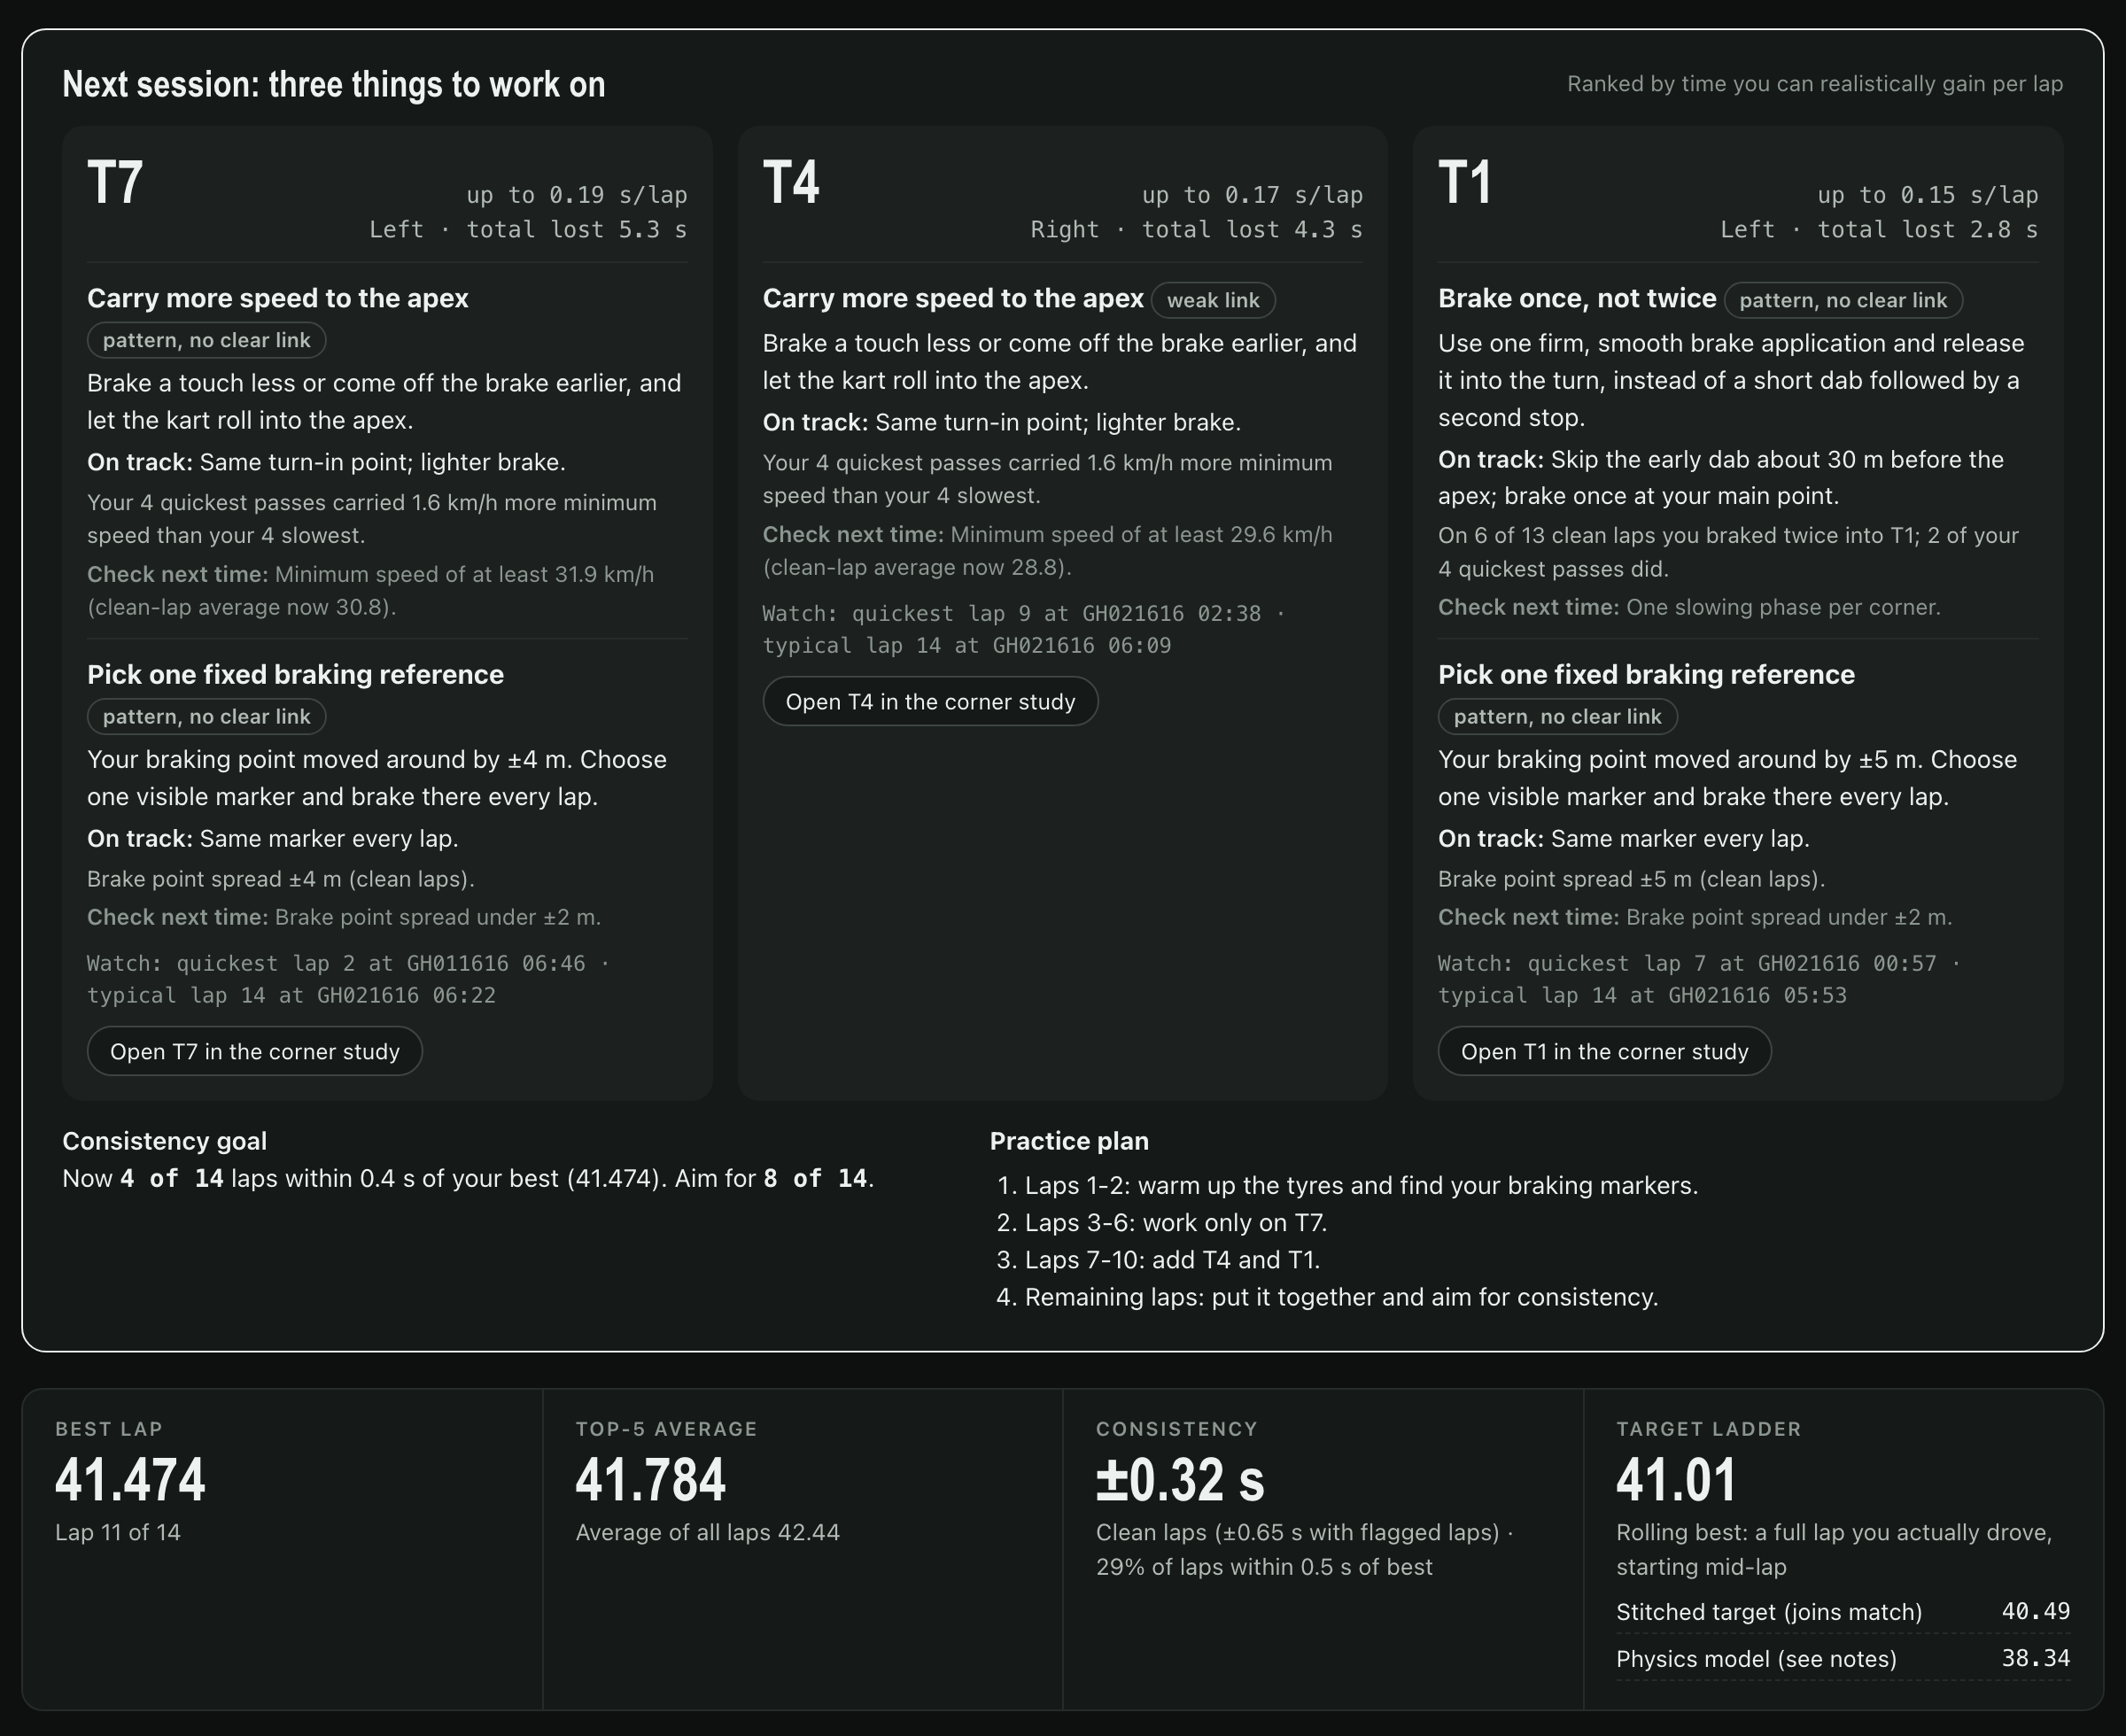
\includegraphics[width=\linewidth,height=0.82\textheight,keepaspectratio]{img/session-debrief.png}
    \end{column}
    \begin{column}{0.35\textwidth}
      \begin{itemize}
        \item Реальна сесія: 14 кіл, «Жага швидкості», GoPro HERO7
        \item Три повороти з порадами й планом на наступний заїзд
        \item Біля кожної поради — момент у відео
      \end{itemize}
    \end{column}
  \end{columns}

  \note{[Доповідач 4] Ось як це виглядатиме. Це макет розбору однієї реальної сесії: 14 кіл на картодромі «Жага швидкості», знято на GoPro HERO7. Угорі — блок «три речі, над якими працювати»: повороти, де можна виграти найбільше часу. Для кожного є порада простими словами і цифра, яку варто перевірити наступного разу, а також посилання на момент у відео. Нижче — план на наступний заїзд і підсумкові цифри сесії. У повному макеті є ще карта траси з межами і таблиця часу по колах. Саме такий результат пілот має отримувати після кожного заїзду.}
\end{frame}

% ===== 11. Ризики =====
\begin{frame}{Ризики і як ми з ними працюємо}
  \centering
  \begin{tabularx}{\textwidth}{@{}>{\raggedright\arraybackslash}p{0.38\textwidth} >{\raggedright\arraybackslash}X@{}}
    \toprule
    \textbf{Ризик зі SWOT} & \textbf{Що робимо в проєкті} \\
    \midrule
    Точність GPS у телефоні \textasciitilde{}4,9 м (W1)
      & Основне джерело — GoPro з GPS, телефон — з попередженням \\
    Точні межі траси потребують фото з дрона (W6)
      & Межі із супутника, невпевнені ділянки — пунктиром \\
    Криті картодроми без GPS (W3)
      & MVP — лише відкриті траси \\
    Tenth Finder і Kart Track уже дають поради (T1)
      & Перевіряємо їх до розробки; ми — без нового обладнання \\
    \bottomrule
  \end{tabularx}

  \note{[Доповідач 4] Звісно, ризики є, і ми їх не ховаємо. Точність GPS у телефоні — близько 4,9 метра. Тому основним джерелом буде відео GoPro з GPS, а трек із телефона підтримаємо з попередженням про точність. Точні межі траси потребують фото з дрона, тож у MVP беремо межі із супутникових знімків, а невпевнені ділянки показуємо пунктиром і порад щодо траєкторії там не даємо. Криті картодроми без GPS у MVP не входять. А конкурентів, Tenth Finder і Kart Track, ми встановимо й перевіримо ще до розробки. Повний список ризиків і рішень є в документі з рішенням.}
\end{frame}

% ===== 12. Наступні кроки =====
\begin{frame}{Наступні кроки}
  \begin{enumerate}
    \setlength{\itemsep}{6pt}
    \item \textbf{Обсяг MVP:} відео GoPro, одна відкрита траса, 2–3 поради
    \item \textbf{Технології:} перевірити gopro-telemetry
    \item \textbf{Методика демо:} що автоматизуємо — межі, зсув GPS
    \item \textbf{Супутникові знімки:} перевірити умови використання
    \item \textbf{Конкуренти:} встановити Tenth Finder і Kart Track
  \end{enumerate}

  \note{[Доповідач 4] Що далі. Спочатку визначаємо обсяг MVP: відео GoPro, одна відкрита траса, поділ на кола, втрати часу по поворотах і дві-три поради. Потім обираємо технології і першою перевіряємо бібліотеку gopro-telemetry. Також розбираємо методику нашого демо і вирішуємо, що з неї робимо автоматично: обведення меж траси за супутником і корекцію зсуву GPS. Окремо треба перевірити умови використання супутникових знімків. І ще до розробки встановлюємо Tenth Finder і Kart Track, щоб зрозуміти, яке обладнання їм потрібне і чим ми від них відрізняємося.}
\end{frame}

% ===== 13. Дякуємо =====
\begin{frame}[standout]
  Дякуємо за увагу!\\[0.3em]
  Запитання?

  \vspace{1.5em}
  \raggedright\footnotesize\mdseries
  Повний SWOT і джерела:\\
  \texttt{docs/stages/stage-1/lap-coach/SWOT.md}\\
  \texttt{docs/stages/stage-1/smart-grocery/SWOT.md}\\
  Рішення, критерії, ризики: \texttt{docs/stages/stage-1/Decision.md}\\
  Макет розбору заїзду: \texttt{docs/stages/stage-1/lap-coach/Karting-session.html}

  \note{[Доповідач 4] Дякуємо за увагу! Коротко ще раз: ми розглянули дві теми, описали їх, зробили SWOT-аналіз, порівняли за п'ятьма критеріями й обрали цифровий тренер для автоспорту. Він виграє за конкурентною перевагою і меншою залежністю від однієї компанії. Внизу слайда — шляхи до файлів із повним SWOT-аналізом, джерелами і документом з рішенням: там є всі цифри, які ми сьогодні називали, з посиланнями. Якщо цікаво, можемо відкрити макет розбору заїзду в браузері. Будемо раді вашим запитанням.}
\end{frame}


\end{document}
